\setauthor{Moritz Eder}

\section{Mockups}

Als Grundlage für die Entwicklung des Design von Relaxoon standen Design-Mockups des Auftraggebers zur Verfügung.

\begin{figure}[H]
    \centering
    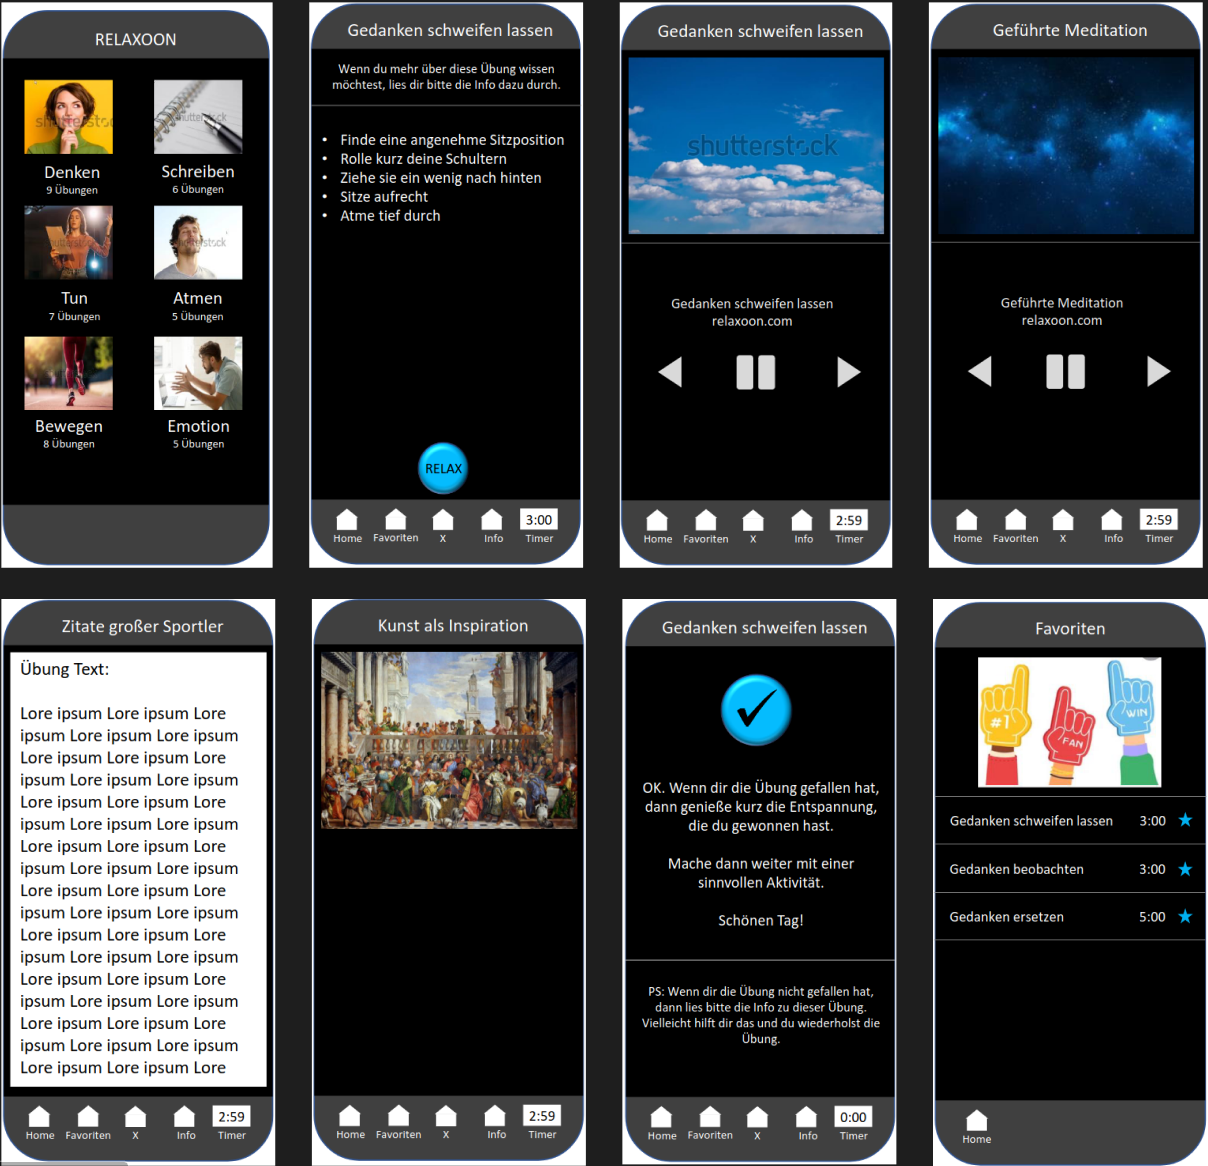
\includegraphics[height=\textwidth]{./pics/mockups.png}
    \caption{Mockups}
\end{figure}

Von oben links bis unten rechts auf dem Bild sind folgende Seiten abgebildet:

\begin{enumerate}
    \item Home-Screen
    \item Übung: Intro
    \item Übung: Video 
    \item Übung: Ton 
    \item Übung: Text 
    \item Übung: Foto 
    \item Übung: Outro
    \item Favoritenliste
\end{enumerate}

\section{Tutorial}

Zu Beginn, wenn man die App zum ersten Mal öffnet, kommt man zu einem Tutorial. Dieses gibt den User:innen einen ersten
Einblick in die App.

Im UI-Prototypen von Relaxoon wurde das Tutorial folgendermaßen realisiert:

\begin{figure}[H]
    \centering
    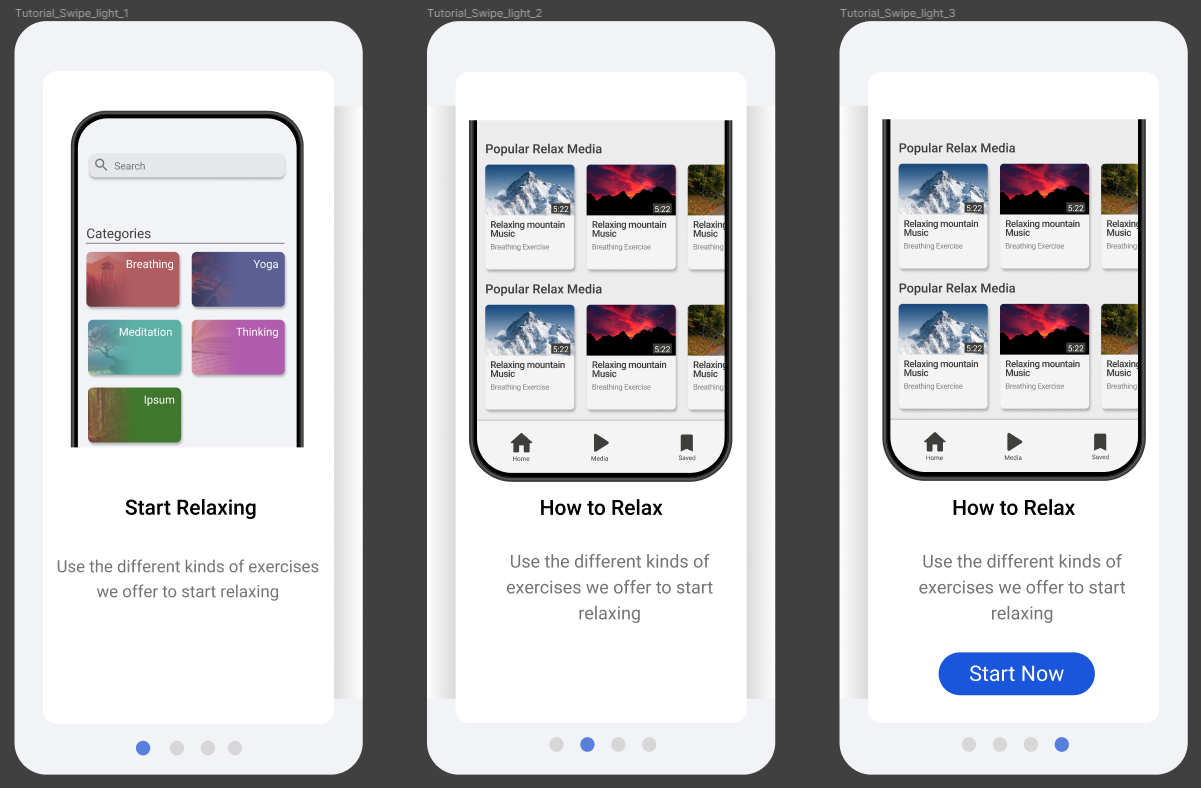
\includegraphics[height=0.65\textwidth]{./pics/pTutorial.png}
    \caption{Tutorial im UI-Prototypen}
\end{figure}

\newpage

Das Konzept wurde bei der Programmierung wie folgt verwirklicht:

\begin{figure}[H]
    \centering
    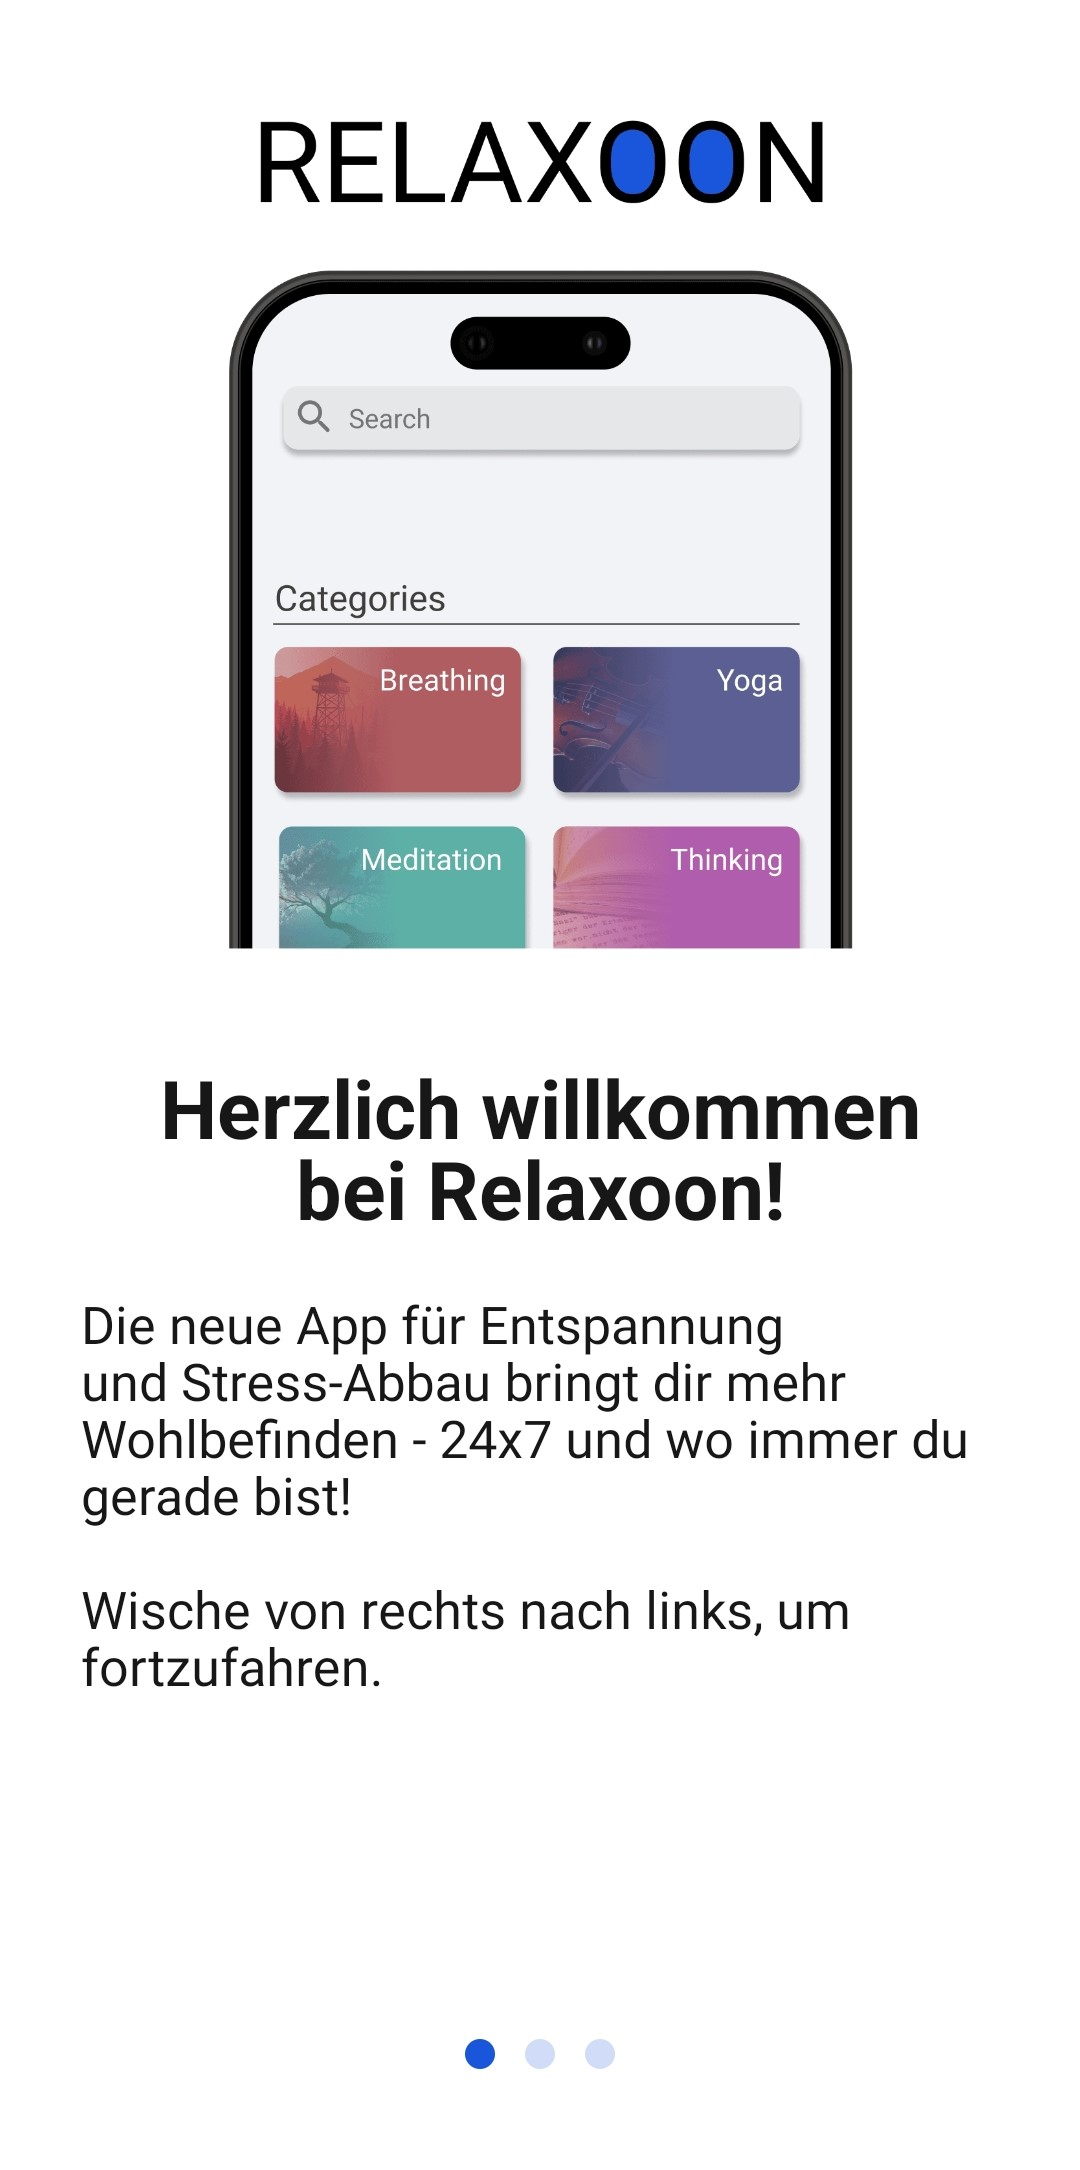
\includegraphics[height=0.71\textwidth]{./pics/Tutorial1.jpg}
    \caption{Erste Tutorial-Page}
\end{figure}
\begin{figure}[H]
    \centering
    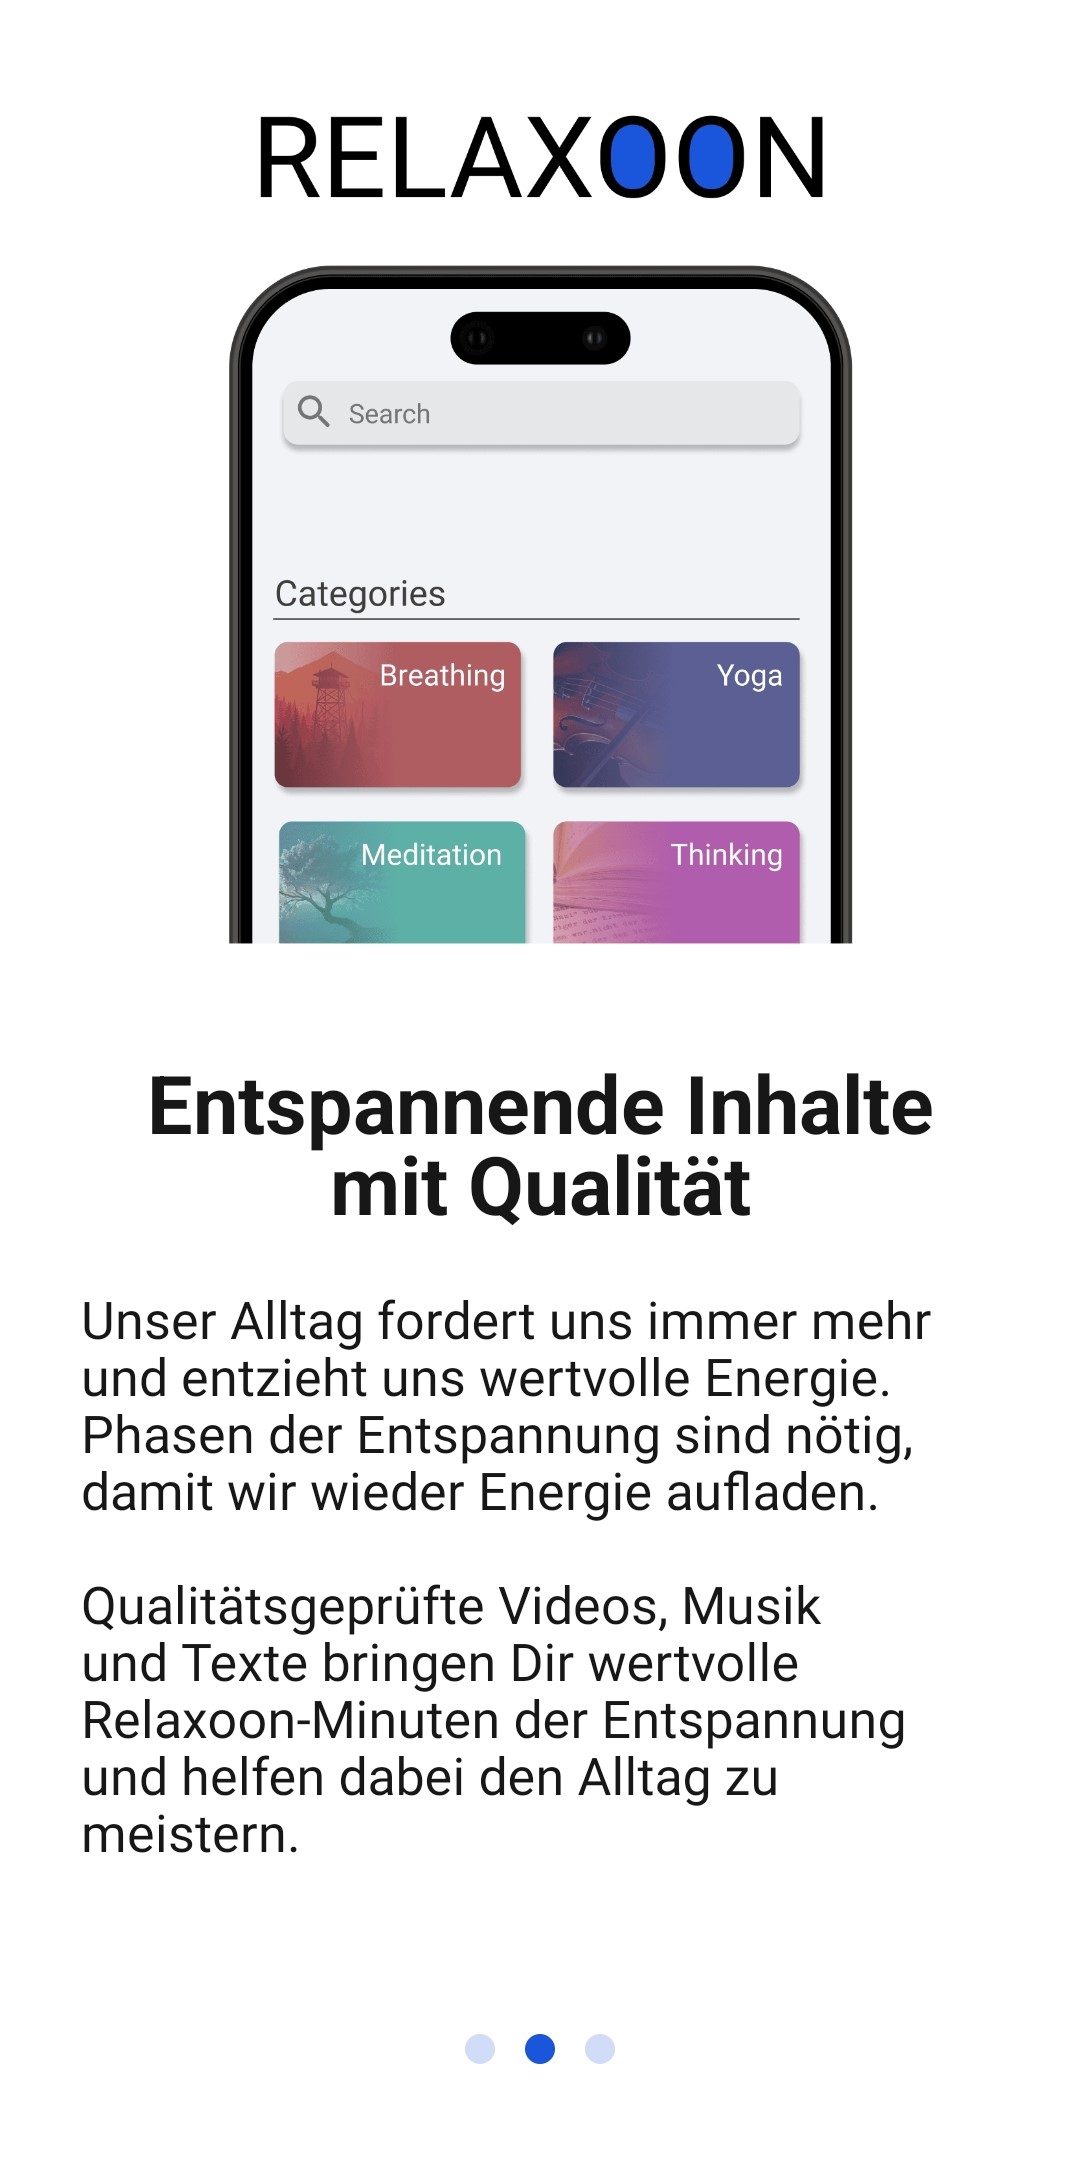
\includegraphics[height=0.71\textwidth]{./pics/Tutorial2.jpg}
    \caption{Zweite Tutorial-Page}
\end{figure}
\begin{figure}[H]
    \centering
    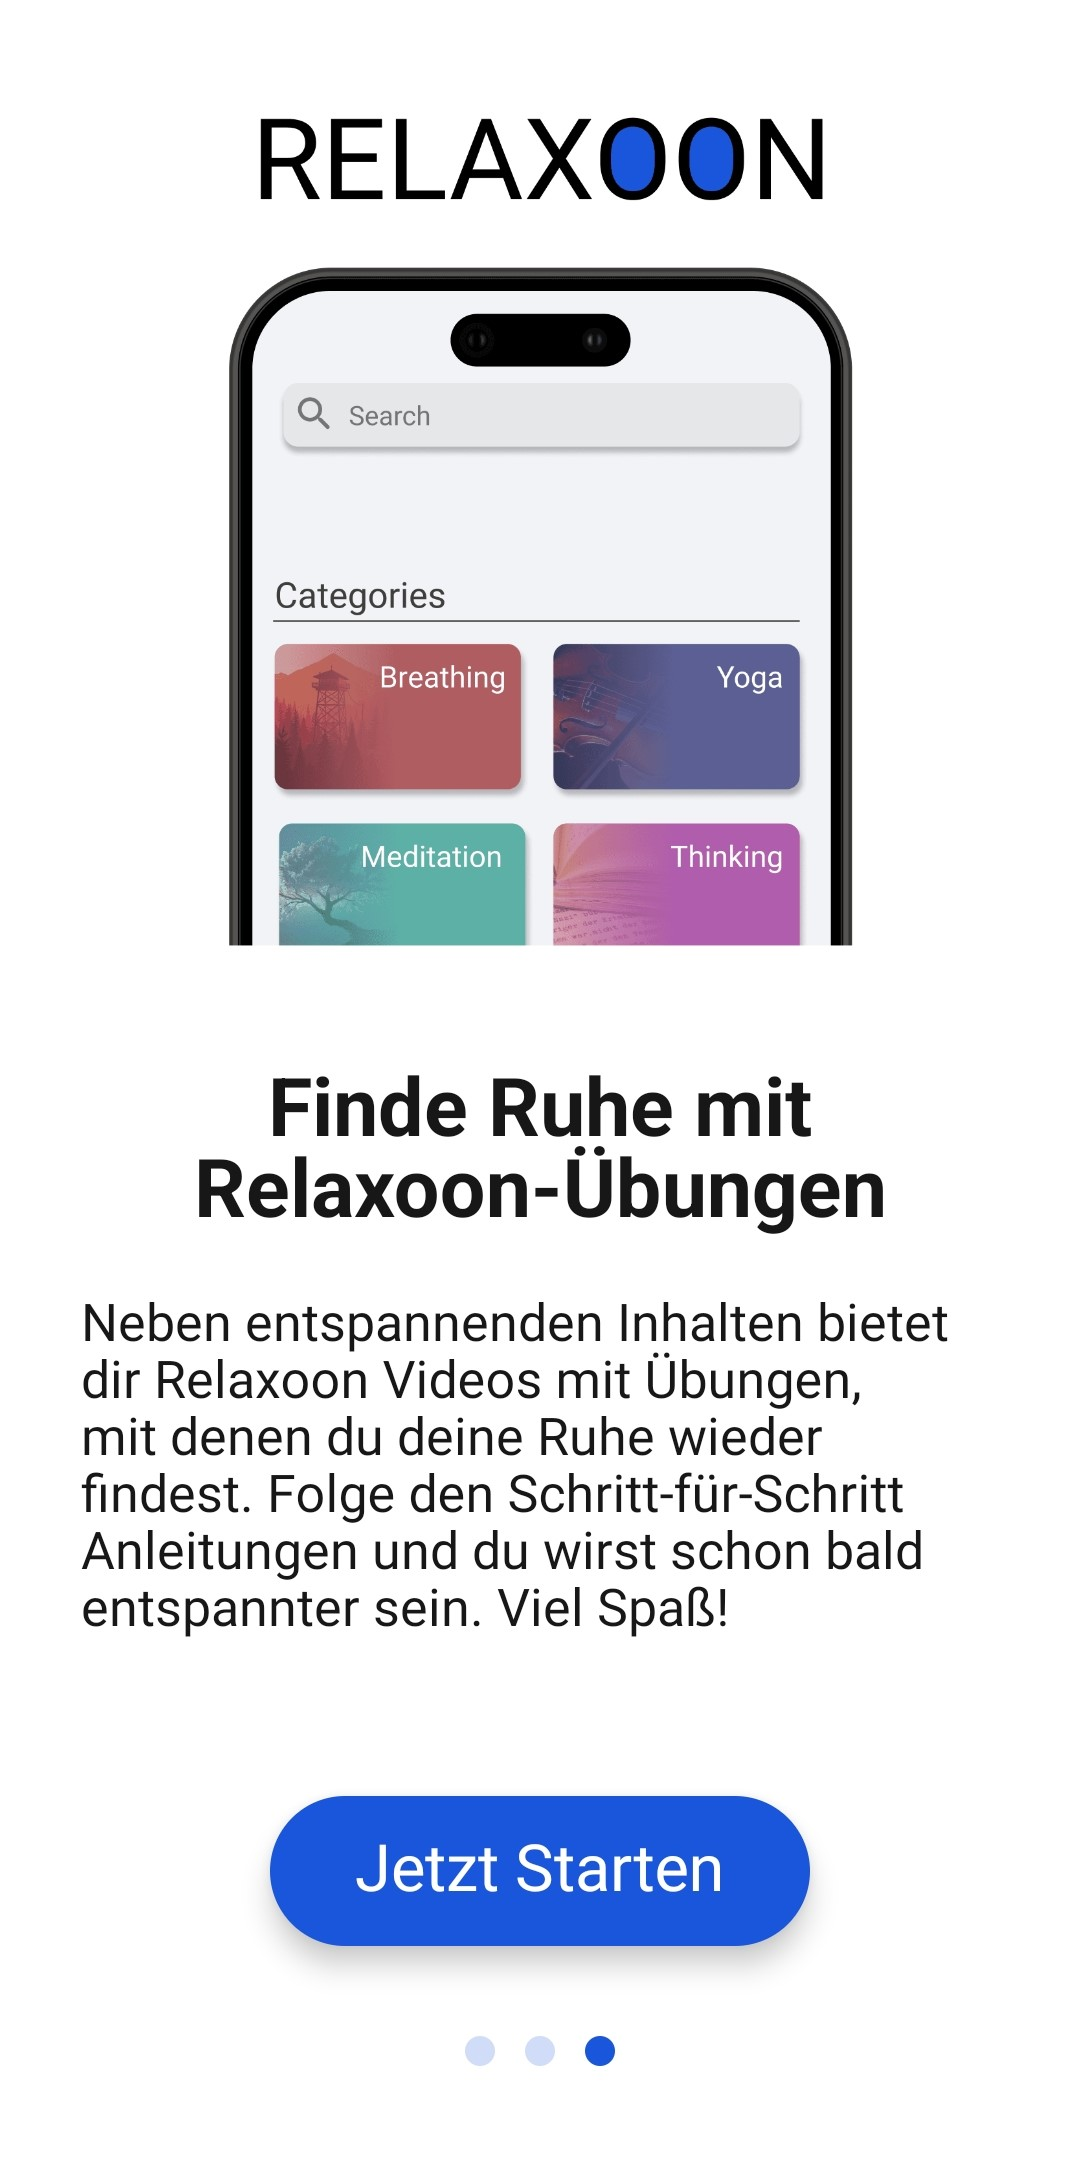
\includegraphics[height=\textwidth]{./pics/Tutorial3.jpg}
    \caption{Dritte Tutorial-Page}
\end{figure}

Auf der letzten Tutorial-Page gelangt man über den ''Jetzt Starten''-Button weiter zum Registrierungsformular.

\section{Login- und Registrierungsformular}

Das Registrierungsformular ist, wie unten dargestellt, nach folgendem Schema aufgebaut:

\begin{enumerate}
    \item Username
    \item E-Mail 
    \item Passwort 
    \item Passwort erneut eingeben
\end{enumerate}

\begin{figure}[H]
    \begin{minipage}{0.5\textwidth}
        \centering
        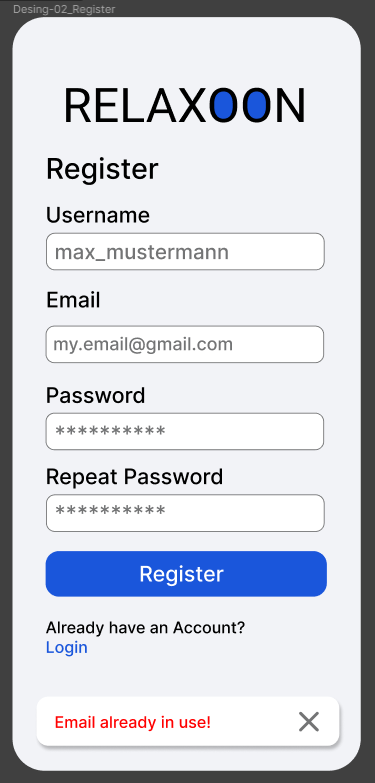
\includegraphics[height=2\textwidth]{./pics/pRegister.png}
        \caption{Registrierung UI-Prototyp}
    \end{minipage}
    \begin{minipage}{0.5\textwidth}
        \centering
        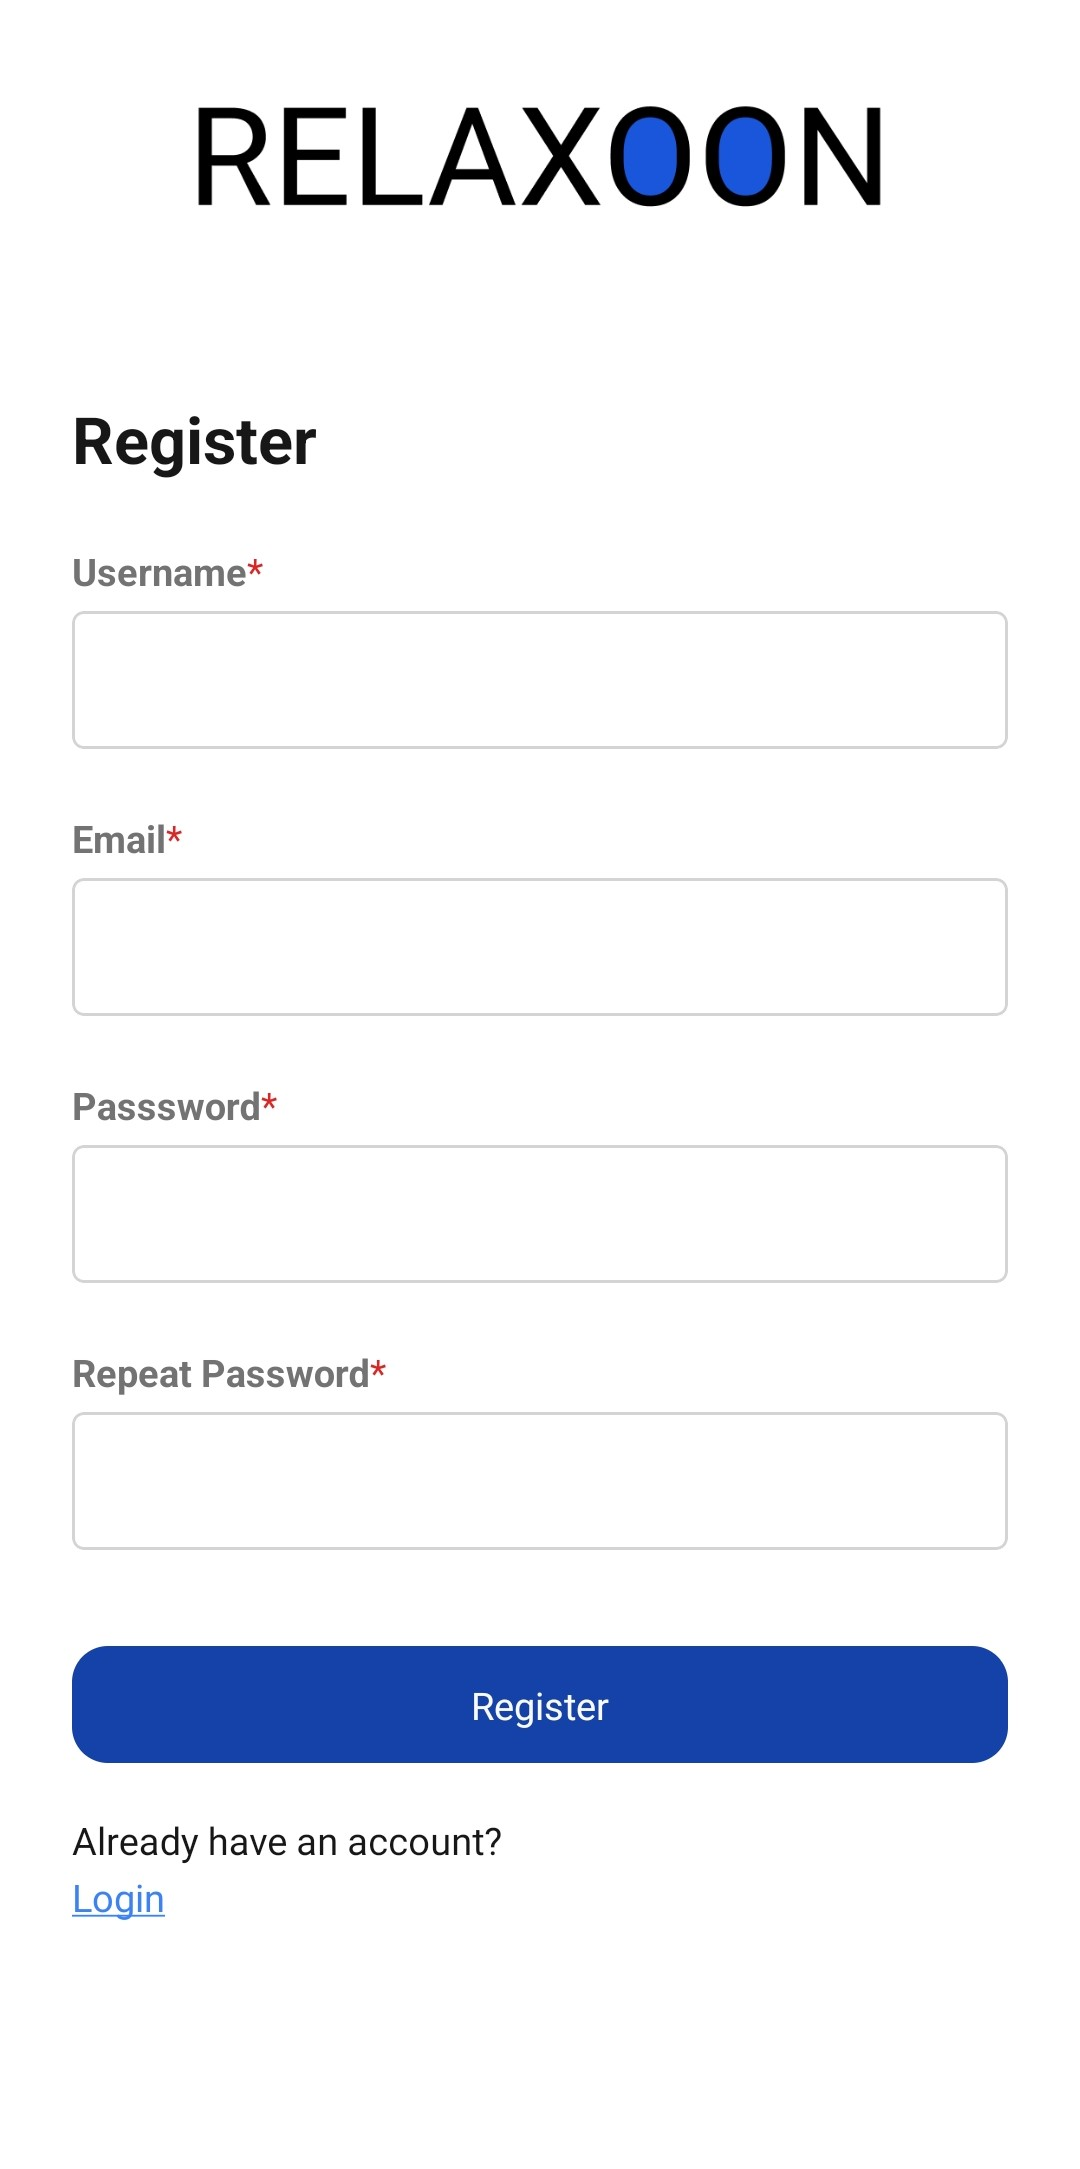
\includegraphics[height=2\textwidth]{./pics/register.jpg}
        \caption{Registrierung in der App}
    \end{minipage}
\end{figure}

Mit dem ''Register''-Button kommt man zum Home-Screen, sofern der Username, die E-Mail und das Passwort korrekt validiert
werden können.

Falls man bereits einen Account besitzt, kann man über das blaue ''Login'' zum Login-Screen navigieren.

\newpage

Um sich einloggen zu können, muss man bei diesem Screen die bereits registrierte E-Mail und das dazugehörige Passwort 
eingeben und auf ''Login'' drücken. Damit gelangt man ebenfalls zum Home-Screen. Über das blaue ''Create an Account''
wird man zurück zur Registrierung geleitet, falls man sich einen neuen Account erstellen will.

\begin{figure}[H]
    \begin{minipage}{0.5\textwidth}
        \centering
        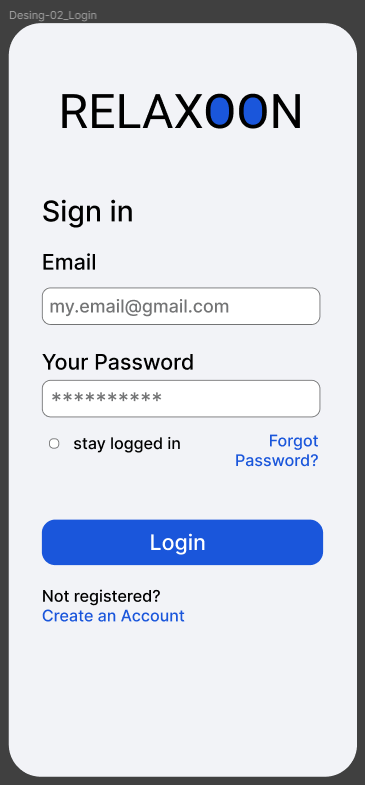
\includegraphics[height=2\textwidth]{./pics/pLogin.png}
        \caption{Login UI-Prototyp}
    \end{minipage}
    \begin{minipage}{0.5\textwidth}
        \centering
        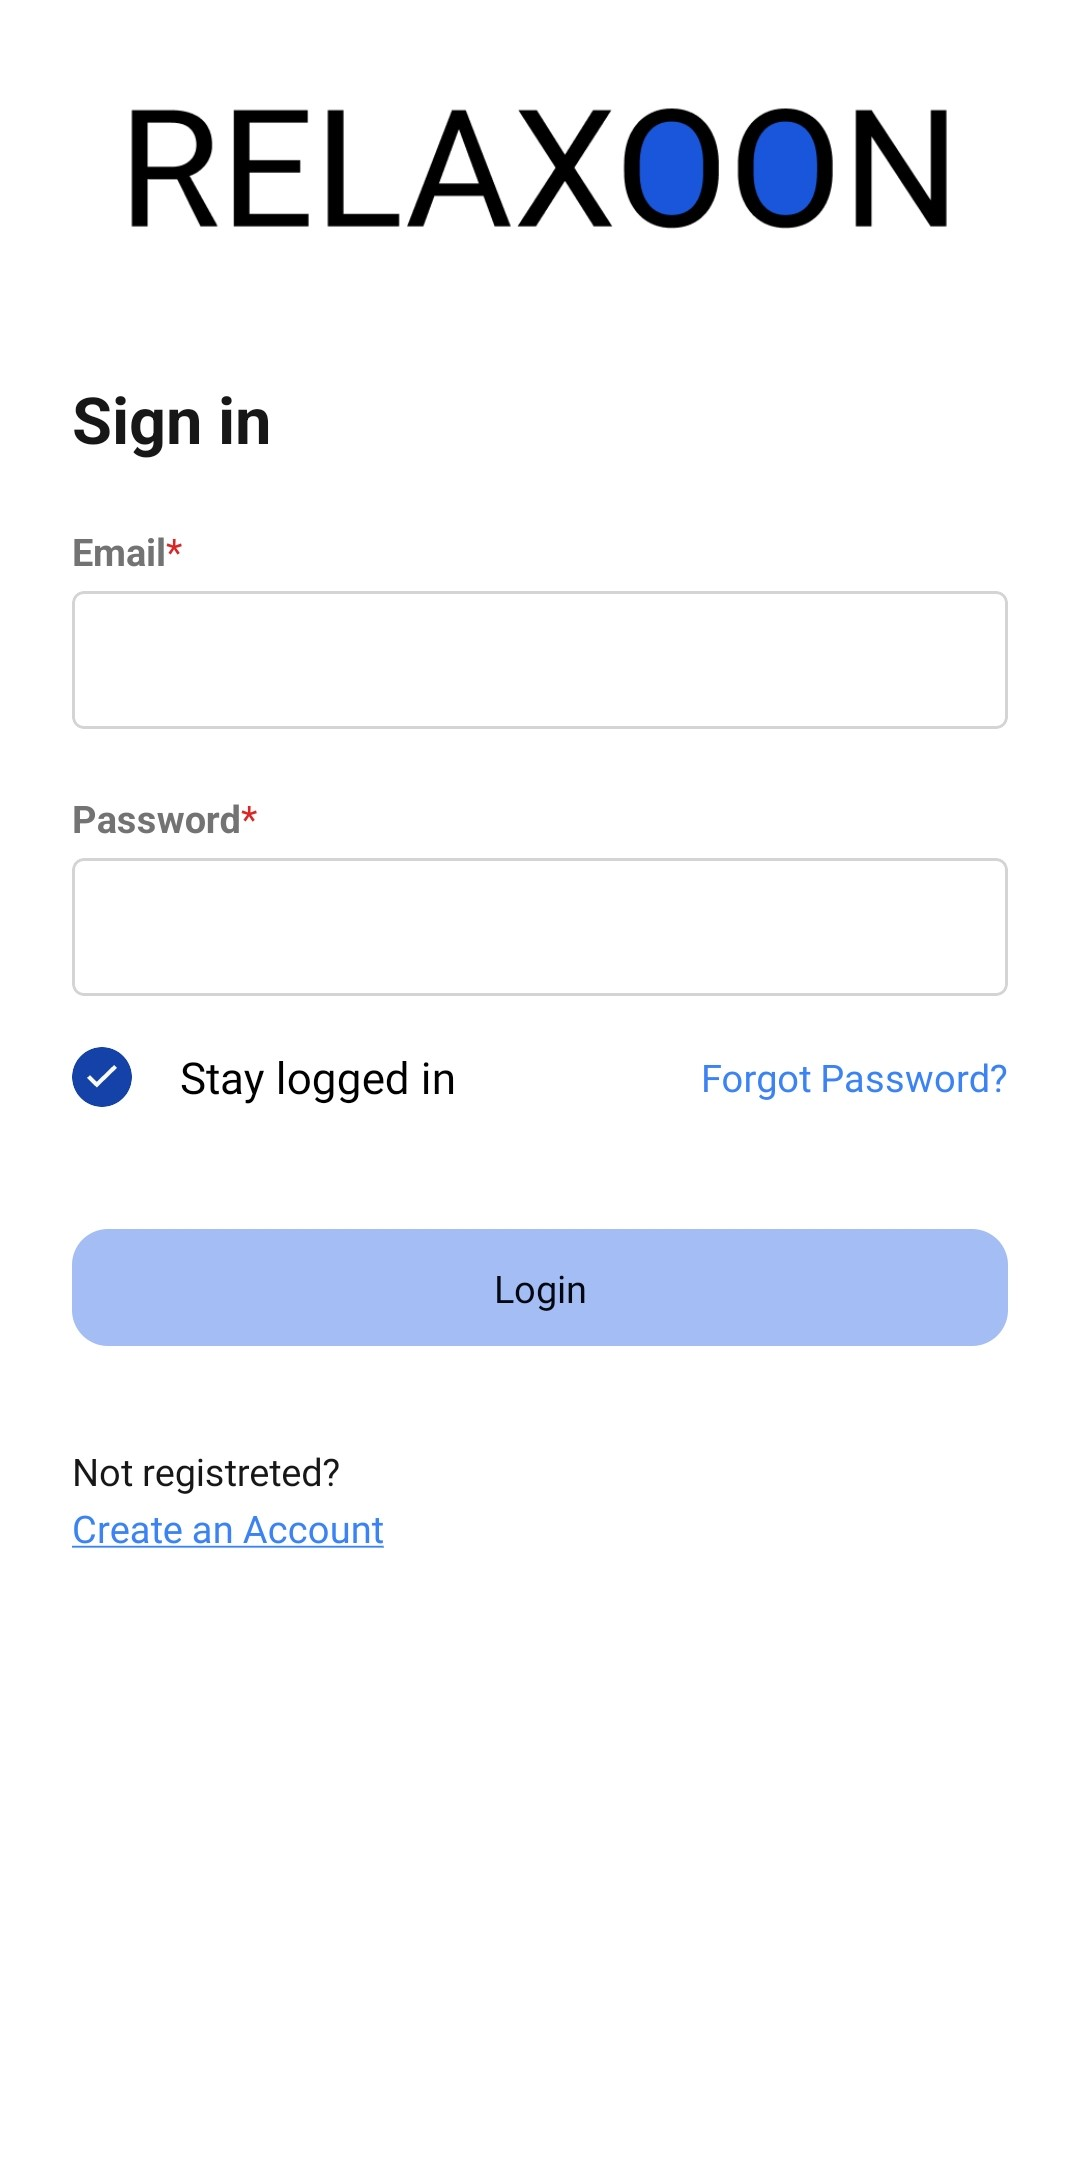
\includegraphics[height=2\textwidth]{./pics/login.jpg}
        \caption{Login in der App}
    \end{minipage}
\end{figure}

Bei erfolgreichem Login wird der/die User:in darüber mit einer Nachricht informiert, die am unteren des Bildschirms 
aufscheint.

\begin{figure}[H]
    \centering
    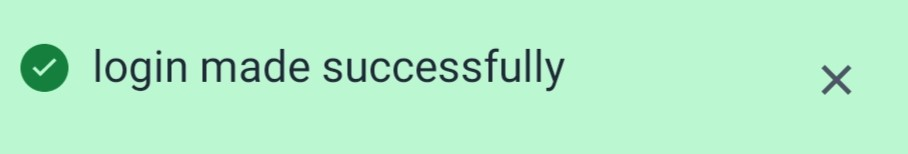
\includegraphics[height=0.09\textwidth]{./pics/message_cut.jpg}
    \caption{Bestätigungsnachricht}
\end{figure}

\section{Home-Screen}

Auf dem Home-Screen ist links oben ein Bereich zu sehen, wo der zuvor eingegebene Username dargestellt wird. Bei drücken
auf das Symbol rechts
oben gelangt man zu den Einstellungen. (siehe Kapitel \ref{chapter:einstellungen})

Unterhalb davon werden eingepflegte Medien vom Backend mit Thumbnail, Titel und einer gekürzten Beschreibung angezeigt.
Auf der Oberfläche ganz unten befindet sich die Navigationsleiste, mit der man zwischen den unterschiedlichen Screens 
navigieren kann.


\begin{figure}[H]
    \begin{minipage}{0.5\textwidth}
        \centering
        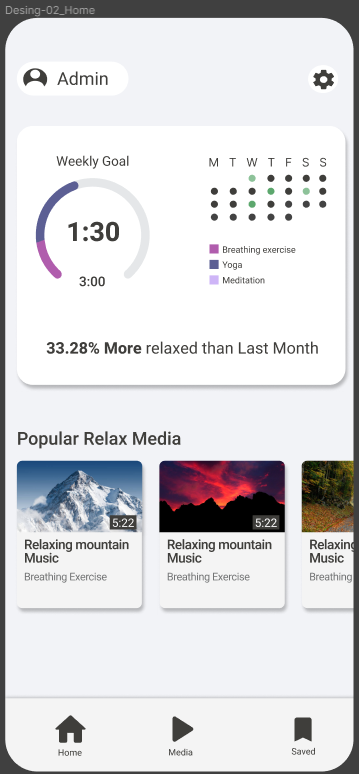
\includegraphics[height=2\textwidth]{./pics/pHome.png}
        \caption{Home-Screen UI-Prototyp}
    \end{minipage}
    \begin{minipage}{0.5\textwidth}
        \centering
        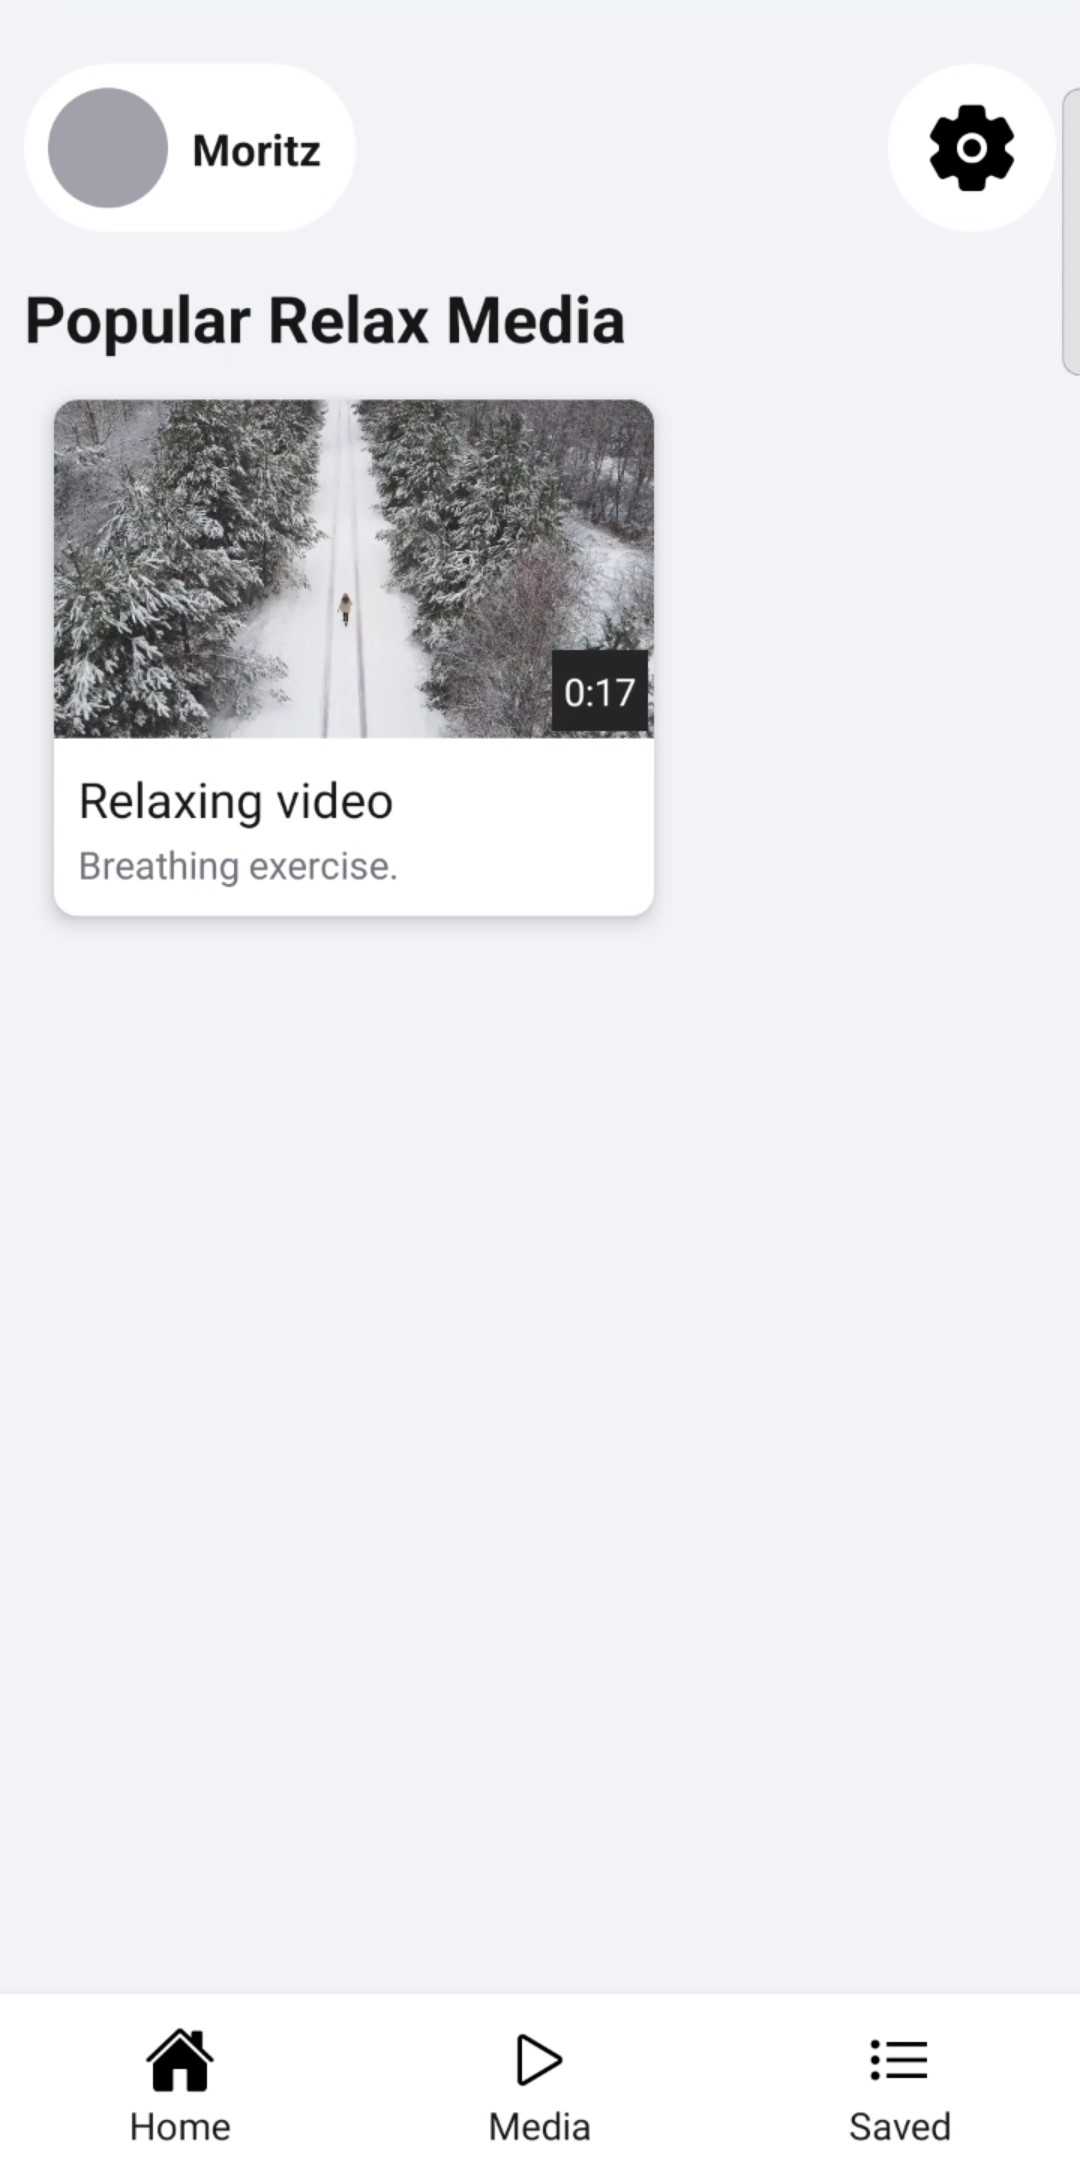
\includegraphics[height=2\textwidth]{./pics/Home.jpg}
        \caption{Home-Screen in der App}
    \end{minipage}
\end{figure}

\section{Kategorien}

Wenn man in der Navigationsleiste unten auf ''Media'' tippt, wird man zu einer Übersicht von Kategorien weitergeleitet.
Hier befindet sich am oberen Rand des Bildschirms die Suchleiste (siehe Kapitel \ref{chapter:suchleiste}) und darunter
werden alle im Backend eingepflegten Kategorien angezeigt. Jede Kategorie hat eine Box, in der der Name der Kategorie
und das Hintergrundbild zu sehen ist.

Durch das Auswählen einer Kategorie kommt man auf die Unterseite, wo die dazugehörigen Medien aufgelistet werden. 

\begin{figure}[H]
    \begin{minipage}{0.5\textwidth}
        \centering
        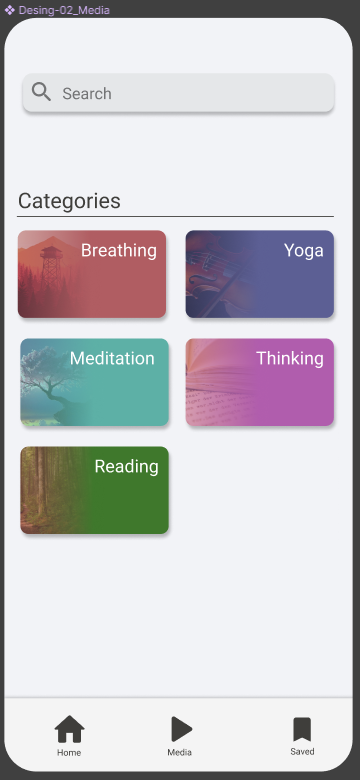
\includegraphics[height=2\textwidth]{./pics/pKategorien.png}
        \caption{Kategorien UI-Prototyp}
    \end{minipage}
    \begin{minipage}{0.5\textwidth}
        \centering
        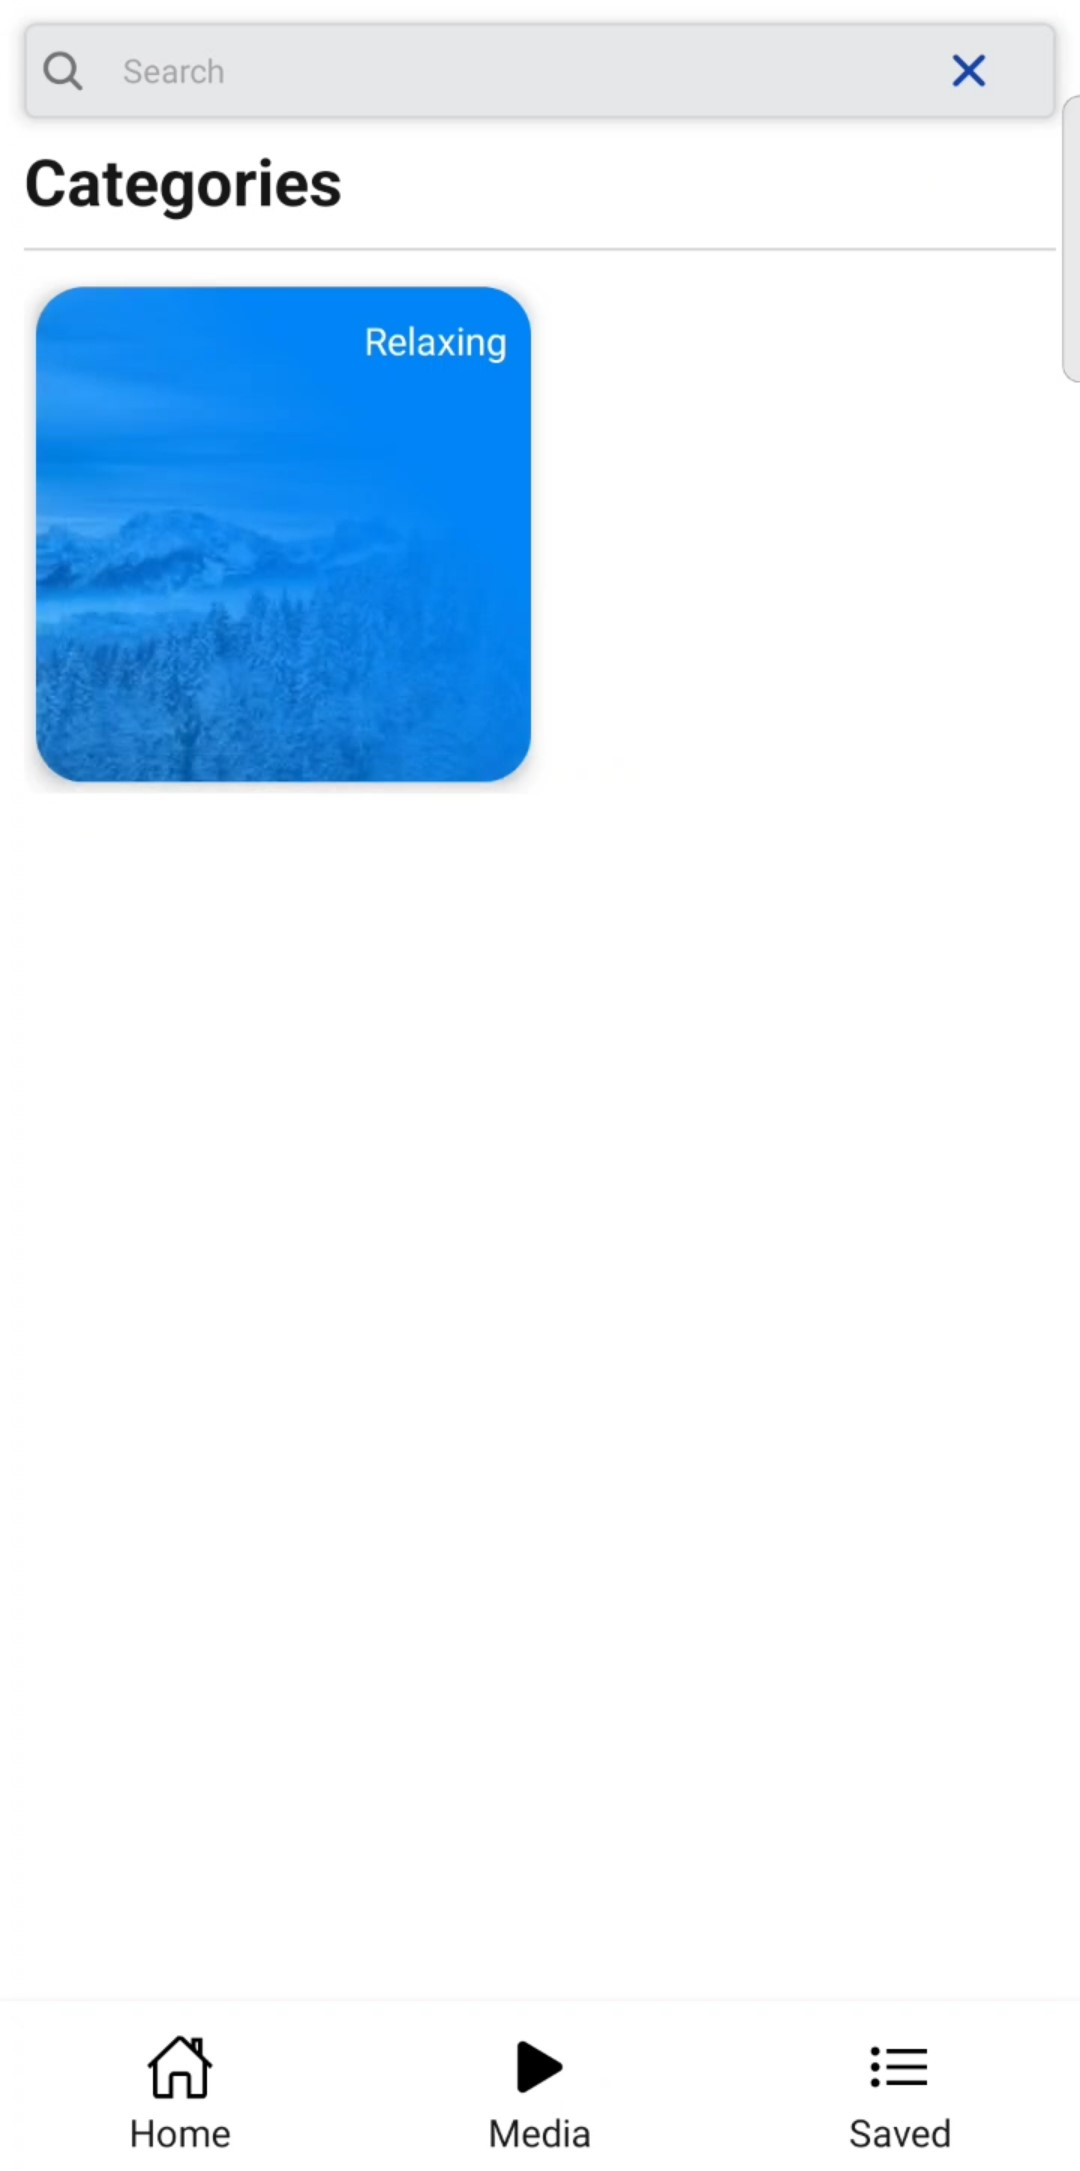
\includegraphics[height=2\textwidth]{./pics/Kategorien.jpg}
        \caption{Kategorien in der App}
    \end{minipage}
\end{figure}

\newpage

Auf der Kategorie-Unterseite befindet sich links oben der ''Zurück-Button''. Dieser leitet den/die User:in wieder 
zurück auf den vorher dargestellten Screen.

Weiters ist der Titel der Kategorie und das Hintergrundbild zu sehen. Darunter werden, wie oben bereits erwähnt, die
dazugehörigen Medien mit Thumbnail, Titel und einer gekürzten Beschreibung aufgelistet.

Rechts daneben ist noch ein 
Stern zu sehen, mit dem man ein Medium als Favorit markieren kann. (siehe Kapitel \ref{chapter:favoriten})

\begin{figure}[H]
    \begin{minipage}{0.5\textwidth}
        \centering
        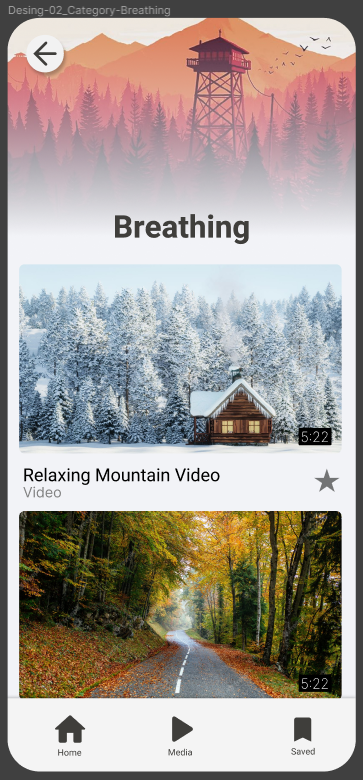
\includegraphics[height=2\textwidth]{./pics/pKategorie.png}
        \caption{Unterseite UI-Prototyp}
    \end{minipage}
    \begin{minipage}{0.5\textwidth}
        \centering
        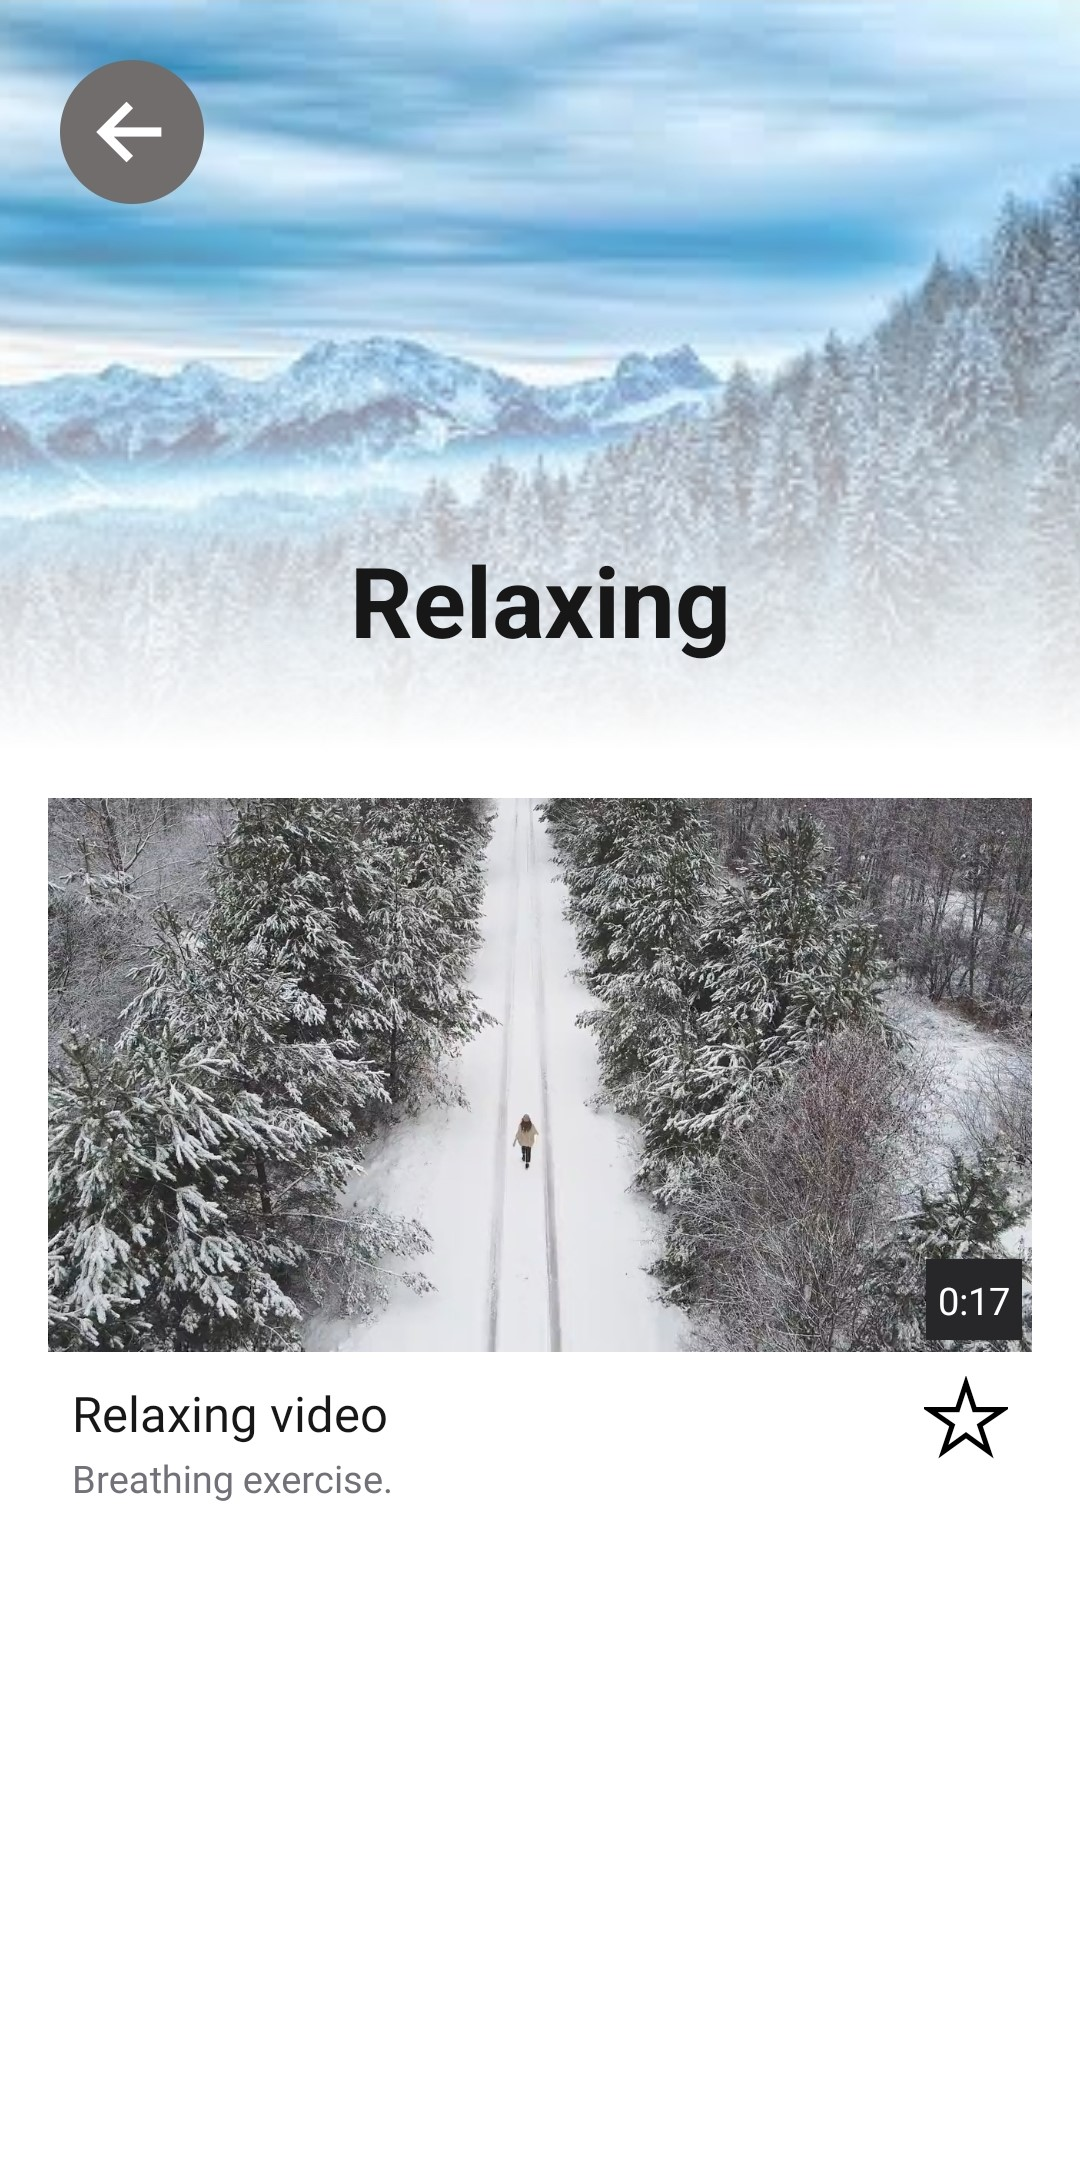
\includegraphics[height=2\textwidth]{./pics/Kategorie.jpg}
        \caption{Unterseite in der App}
    \end{minipage}
\end{figure}

\section{Media Player}

Wenn man ein Video auswählt, wird man zum Media Player weitergeleitet. Dieser bietet die
Funktionen ein Video abzuspielen, zurückzuspulen und vorzuspulen. Man kann das Video auch vergrößern und sich auf dem
Smartphone waagrecht anschauen.

Unter dem Media Player ist der Titel, der Stern zum Markieren eines Favoriten und die Beschreibung abgebildet.
Wenn man ein Video als Favorit markiert, wird der Stern ausgefüllt.

\begin{figure}[H]
    \begin{minipage}{0.5\textwidth}
        \centering
        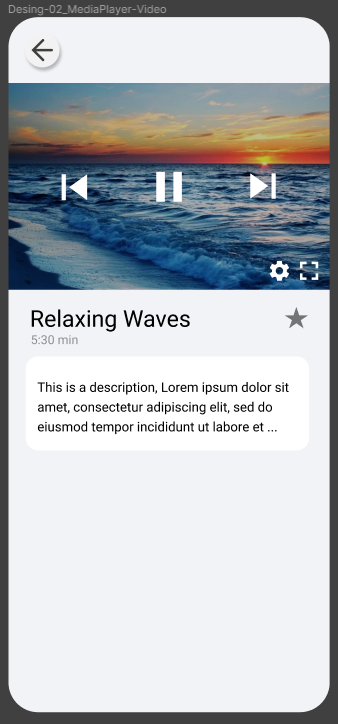
\includegraphics[height=2\textwidth]{./pics/pMediaPlayer.png}
        \caption{Media Player UI-Prototyp}
    \end{minipage}
    \begin{minipage}{0.5\textwidth}
        \centering
        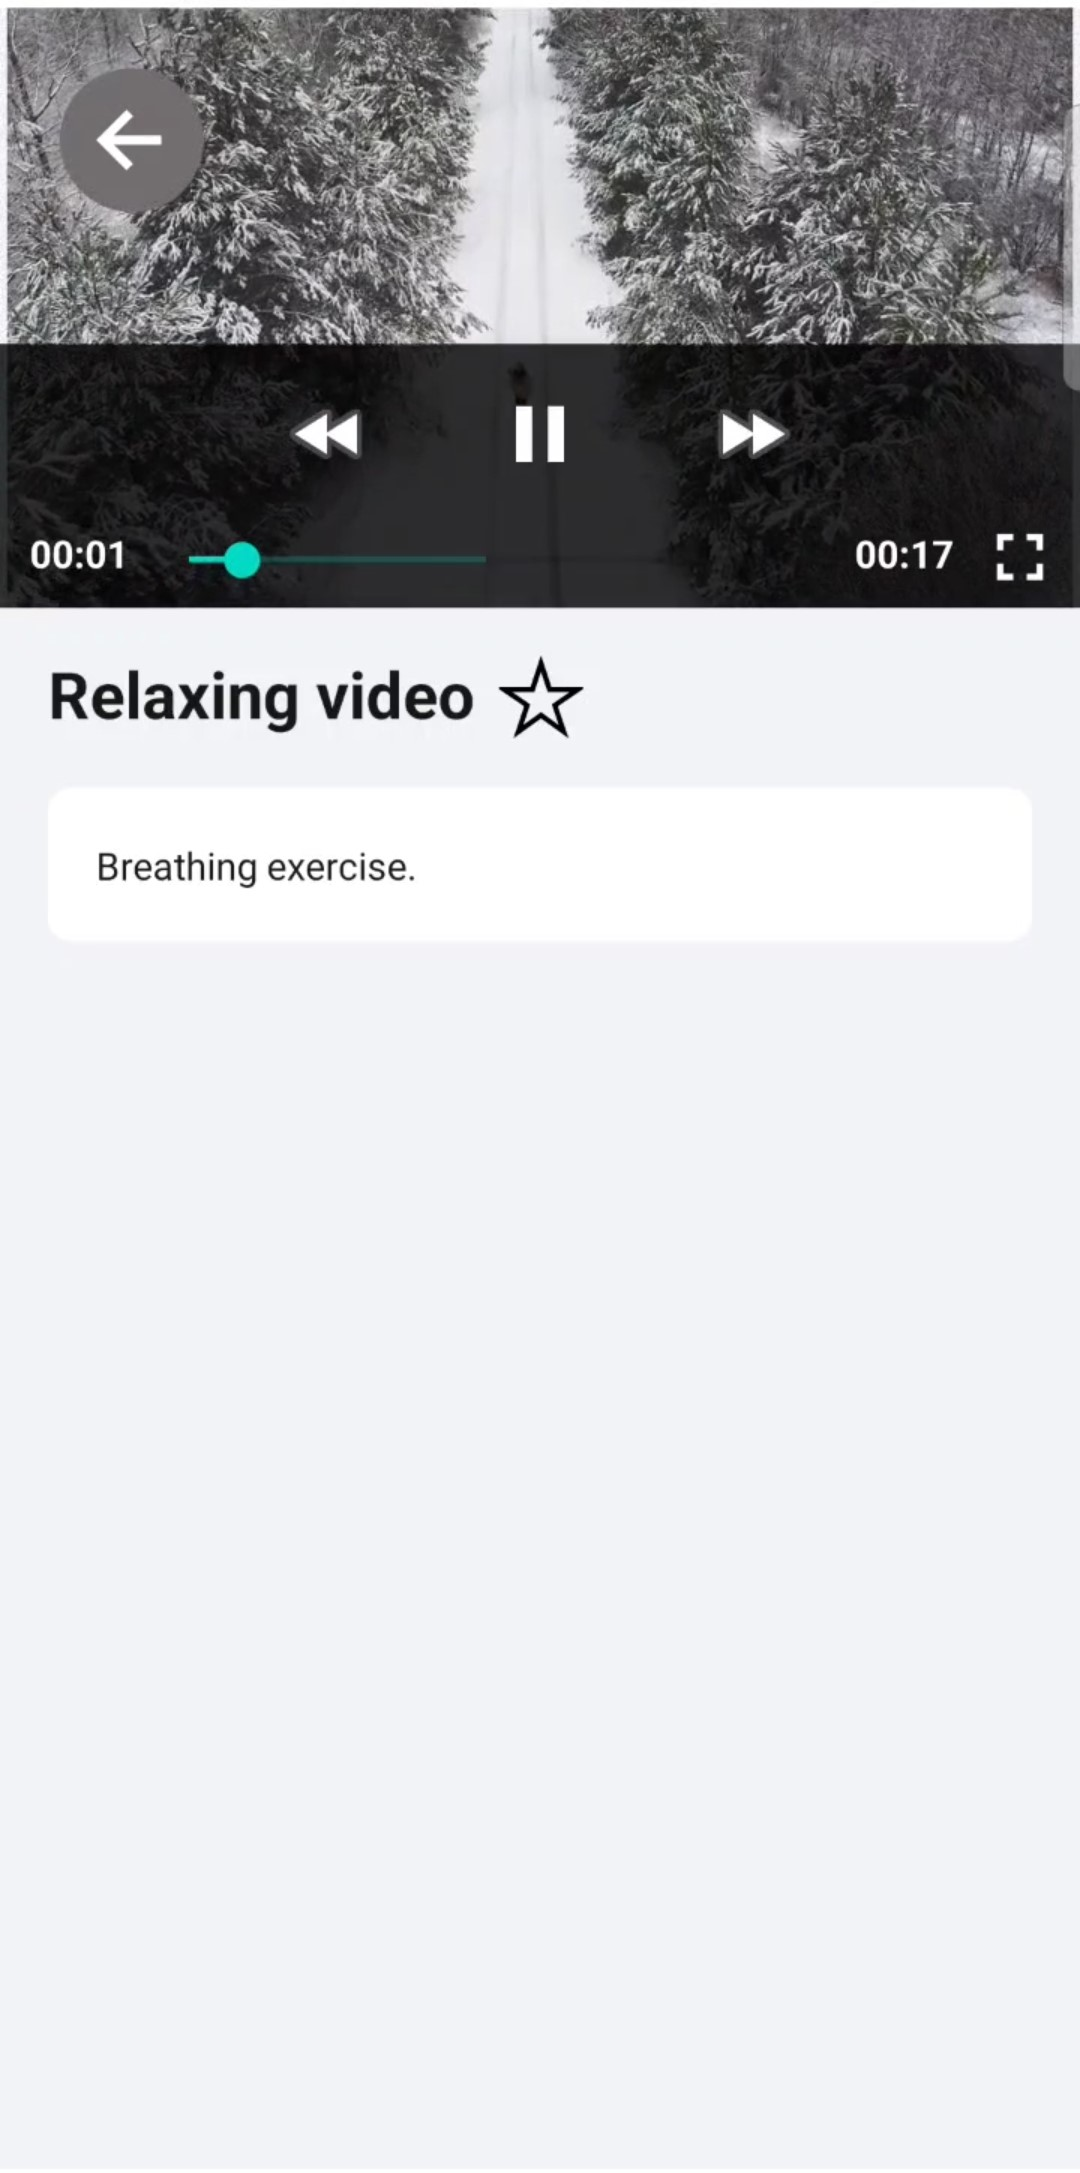
\includegraphics[height=2\textwidth]{./pics/MediaPlayer.jpg}
        \caption{Media Player in der App}
    \end{minipage}
\end{figure}

\newpage

\section{Suchleiste}\label{chapter:suchleiste}

Mit der Suchleiste kann man direkt nach einem Video suchen. Wenn man auf das vorgeschlagene Ergebnis tippt, wird man
direkt zum Media Player weitergeleitet.

\begin{figure}[H]
    \centering
    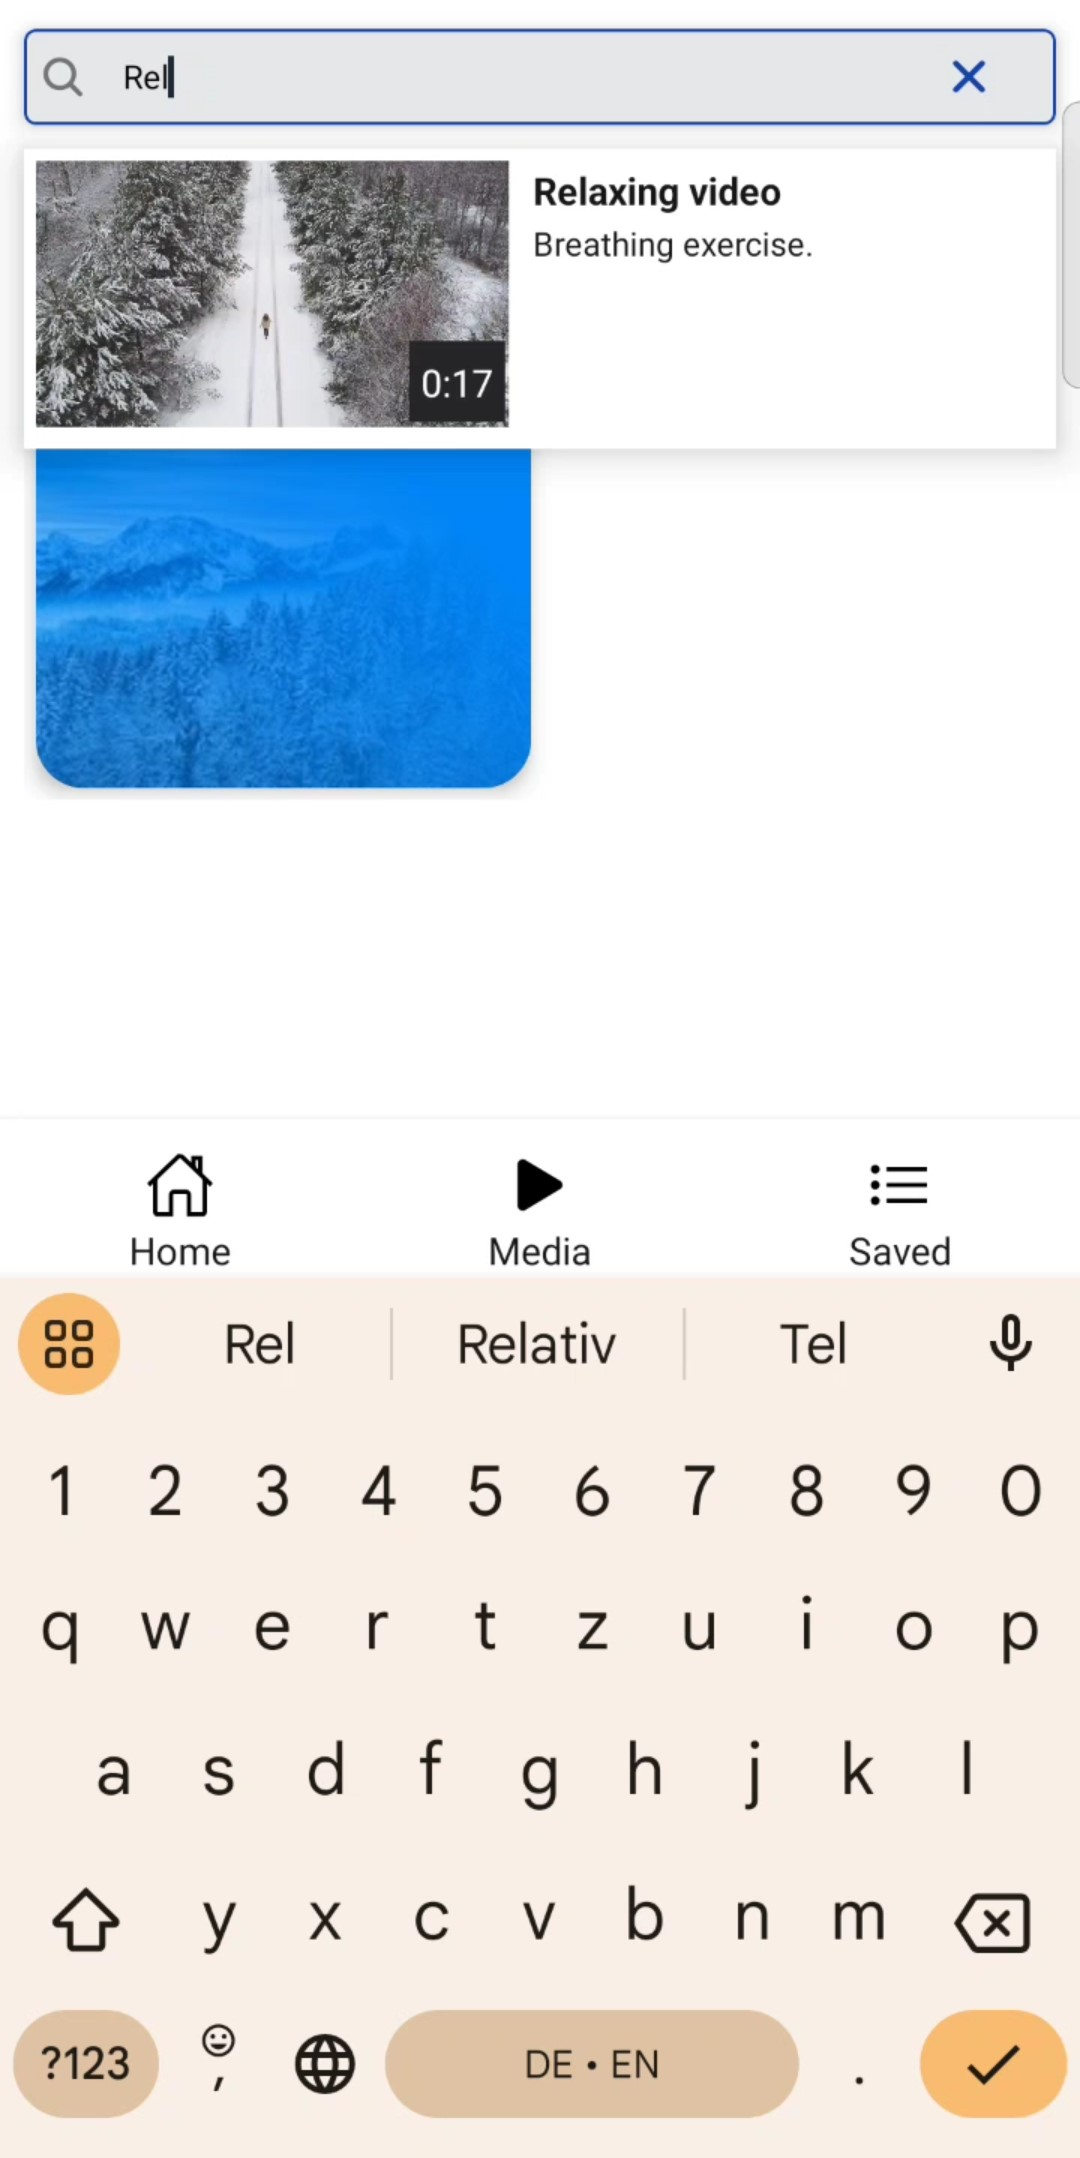
\includegraphics[height=\textwidth]{./pics/Suche.jpg}
    \caption{Suchleiste}
\end{figure}

\newpage

\section{Favoriten}\label{chapter:favoriten}

Die favorisierten Medien werden auf der ''Saved-Page'' aufgelistet, die man in der Navigationsleiste findet.

\begin{figure}[H]
    \centering
    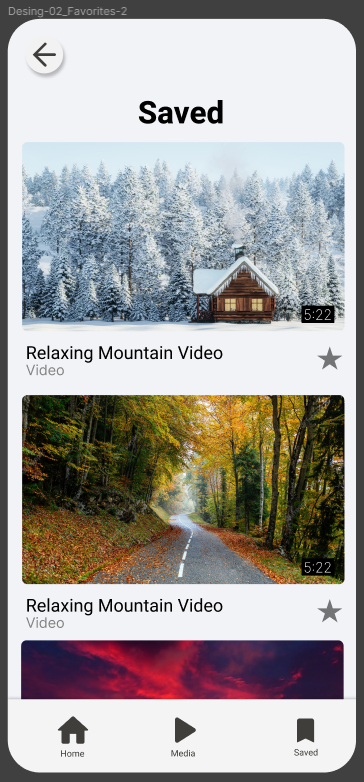
\includegraphics[height=\textwidth]{./pics/pFavoriten.png}
    \caption{Favoriten UI-Prototyp}
\end{figure}

\newpage

Wenn man als User:in noch keinen Favoriten gesetzt hat, erscheint die Nachricht: ''You have no favorites yet''.

Einen Favoriten kann man direkt auf der Favoritenseite durch das Antippen des Sterns wieder löschen, oder auch wenn
man im Media Player auf den ausgefüllten Stern tippt. 

\begin{figure}[H]
    \begin{minipage}{0.5\textwidth}
        \centering
        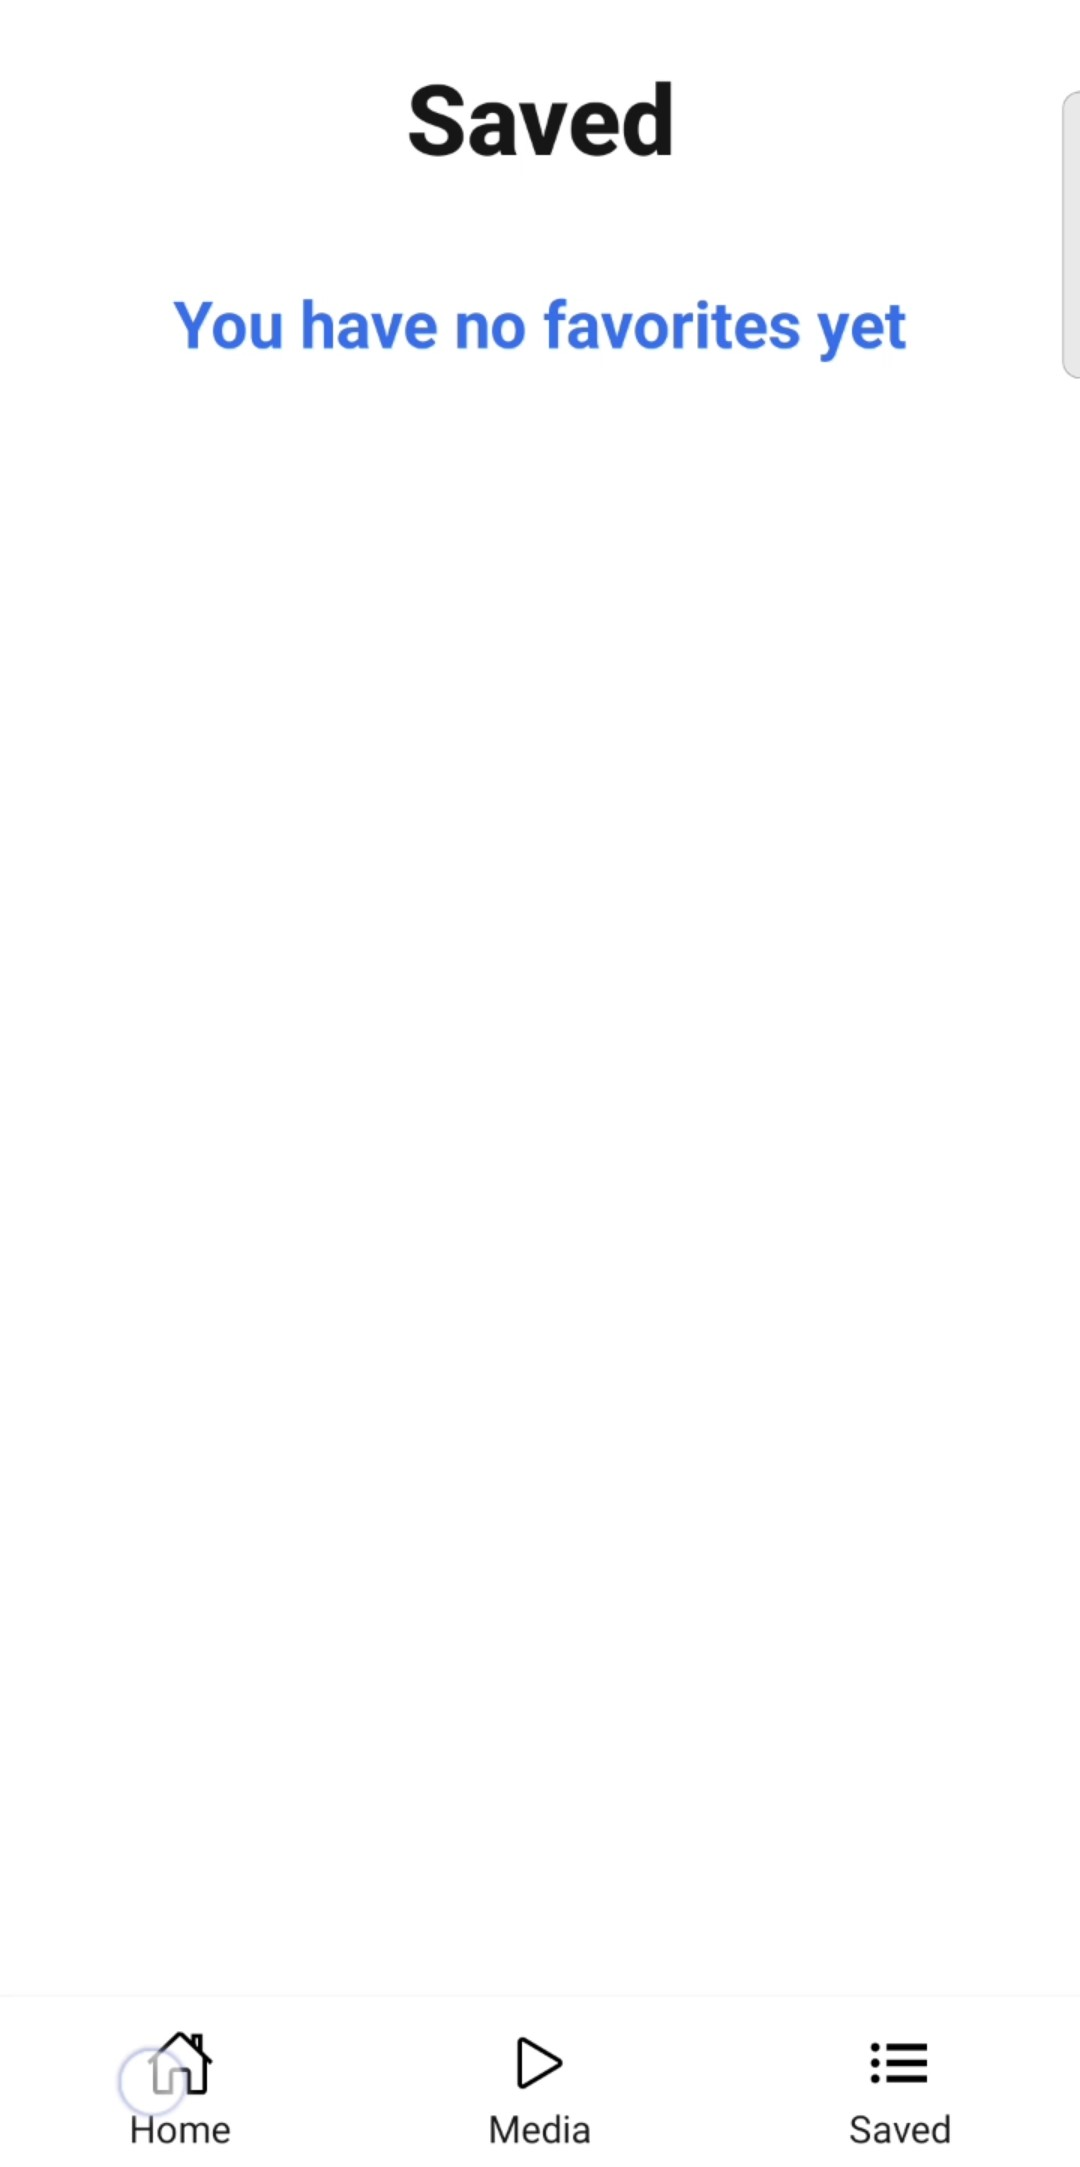
\includegraphics[height=2\textwidth]{./pics/No Favoriten.jpg}
        \caption{Kein Favorit gesetzt}
    \end{minipage}
    \begin{minipage}{0.5\textwidth}
        \centering
        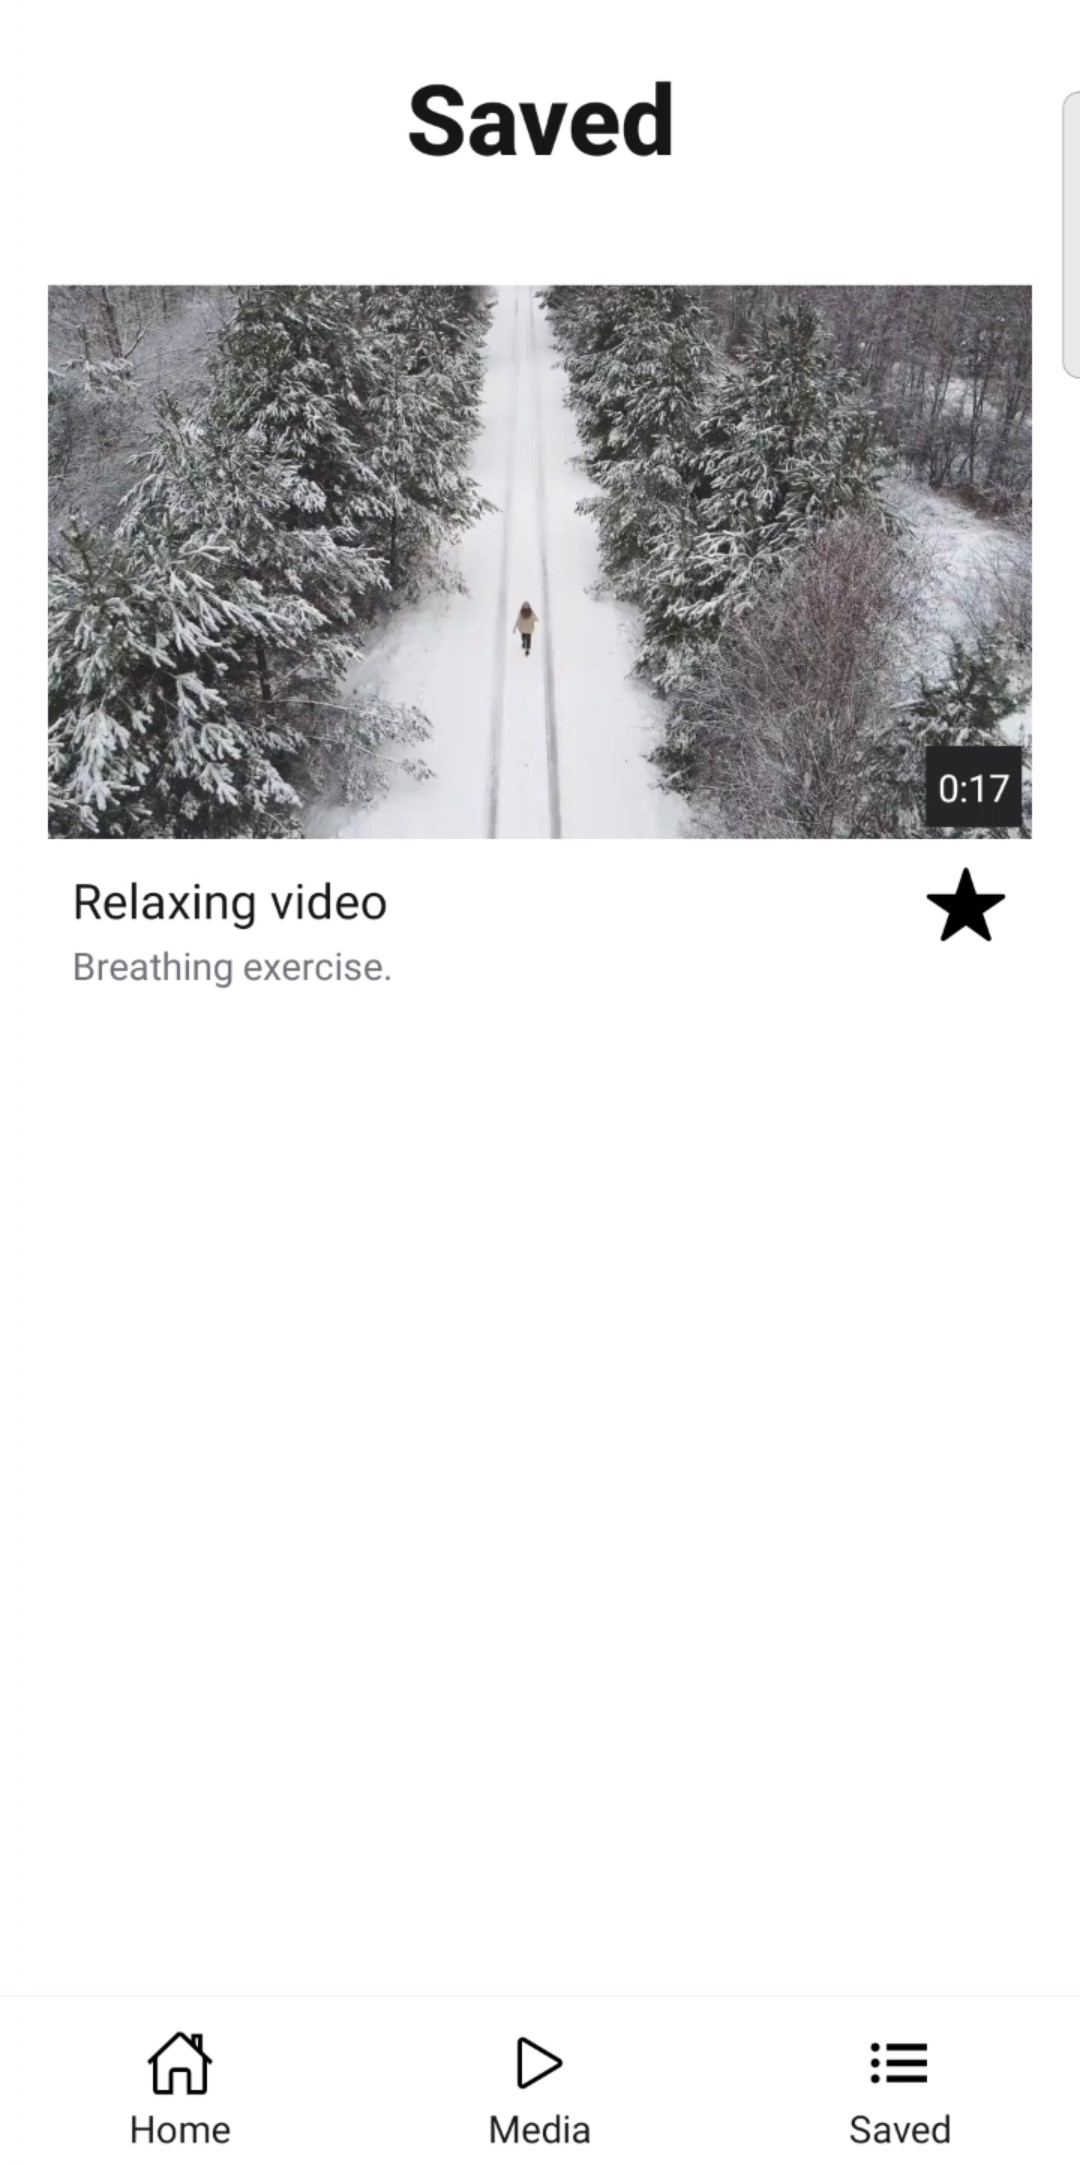
\includegraphics[height=2\textwidth]{./pics/Favoriten.jpg}
        \caption{Ein Favorit gesetzt}
    \end{minipage}
\end{figure}

\newpage

\section{Einstellungen}\label{chapter:einstellungen}

In den Einstellungen ist neben dem ''Zurück-Button'' auch ein Schalter zu finden, mit dem man das Aussehen von Relaxoon
verändern kann. Es wird zwischen Light Mode und Dark Mode unterschieden. (siehe Kapitel \ref{chapter:modes})

Eine Info- und Helpfunktion sind auch verfügbar.

\begin{figure}[H]
    \centering
    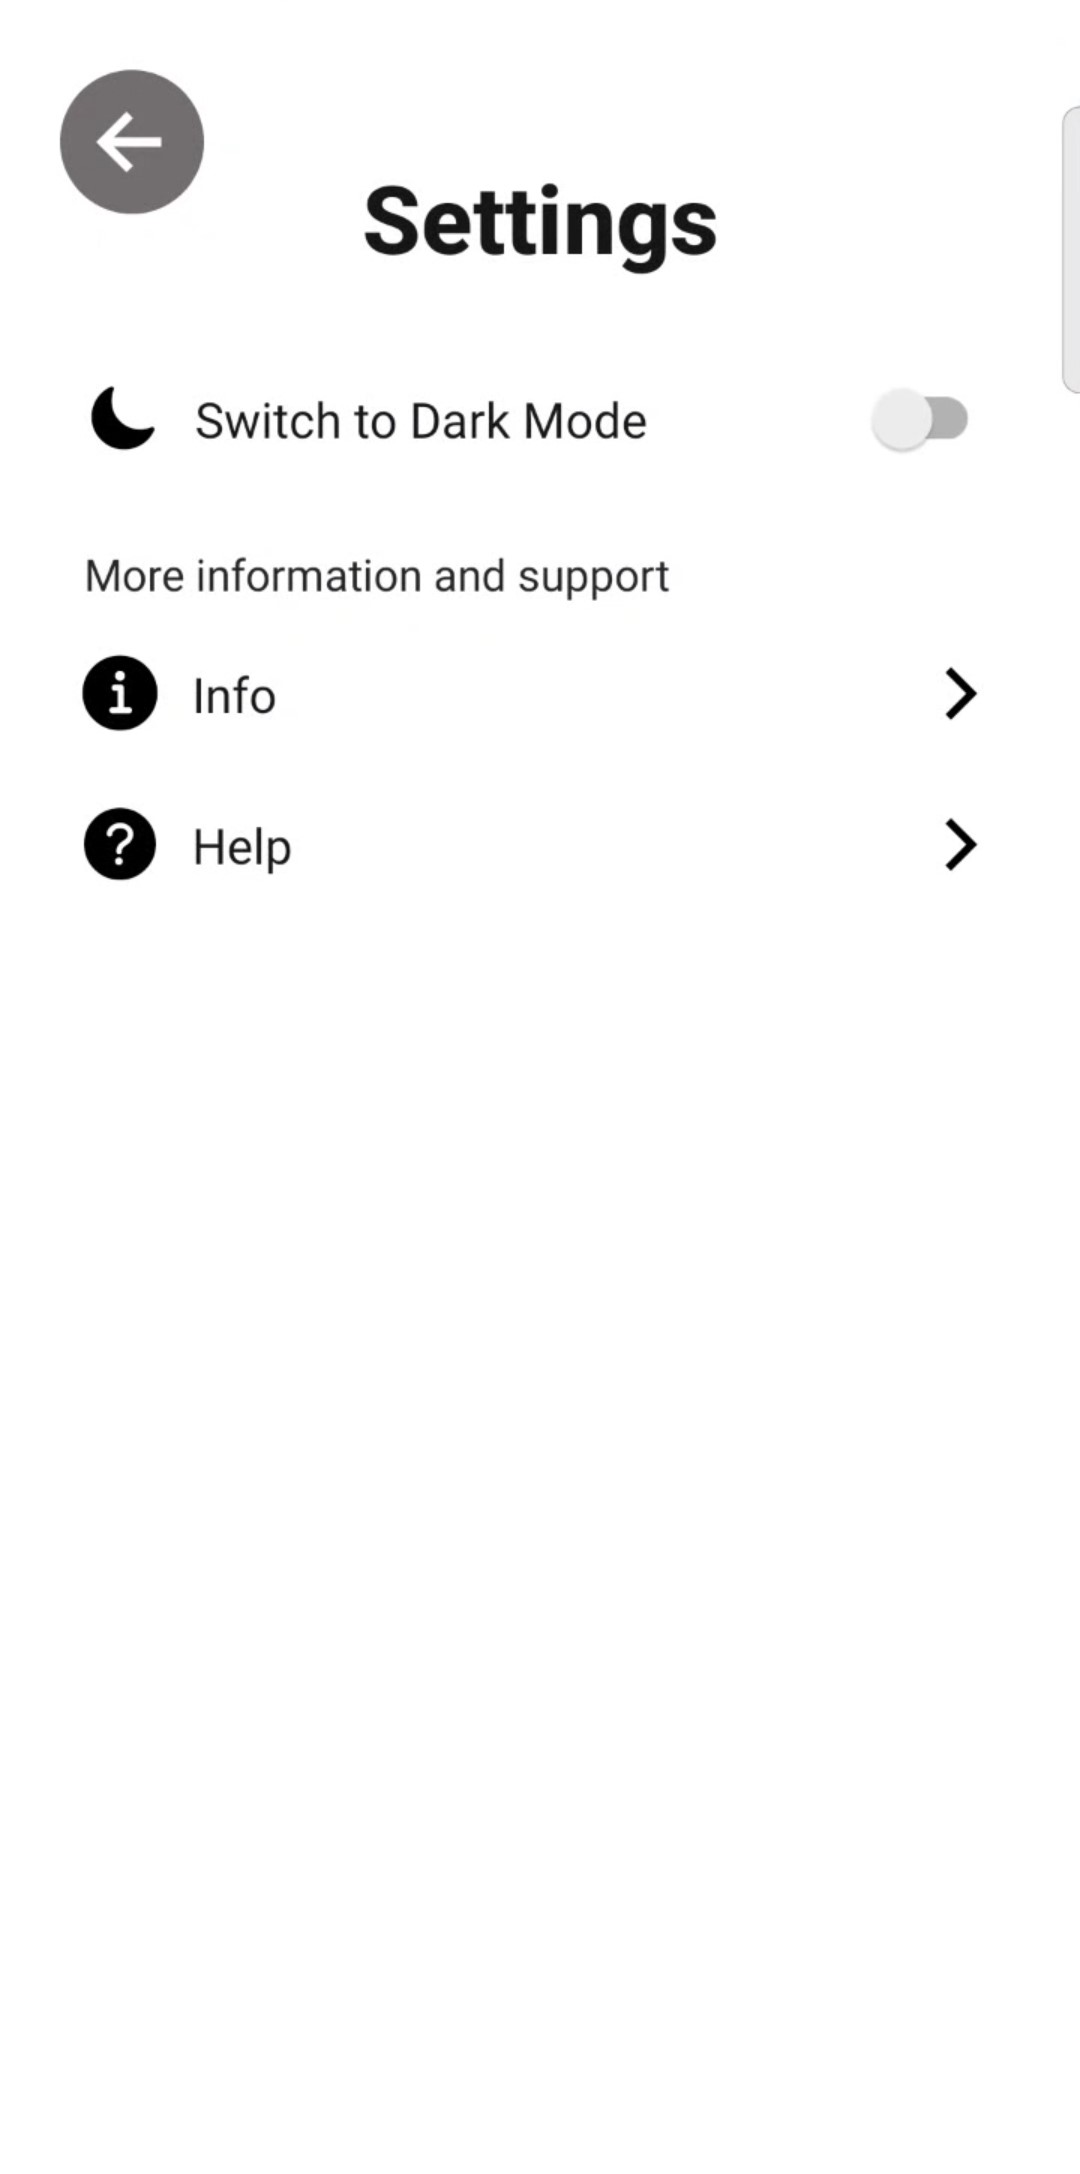
\includegraphics[height=\textwidth]{./pics/Settings.jpg}
    \caption{Einstellungen in der App}
\end{figure}

\newpage

\section{Light/Dark Mode}\label{chapter:modes}

Der Light Mode und Dark Mode bieten dem Benutzer die Möglichkeit, das Erscheinungsbild der App entsprechend der eigenen
Vorlieben oder den Umgebungsbedingungen anzupassen. Im Anschluss sind Screenshots von Relaxoon im Dark Mode abgebildet.

\begin{figure}[H]
    \begin{minipage}{0.5\textwidth}
        \centering
        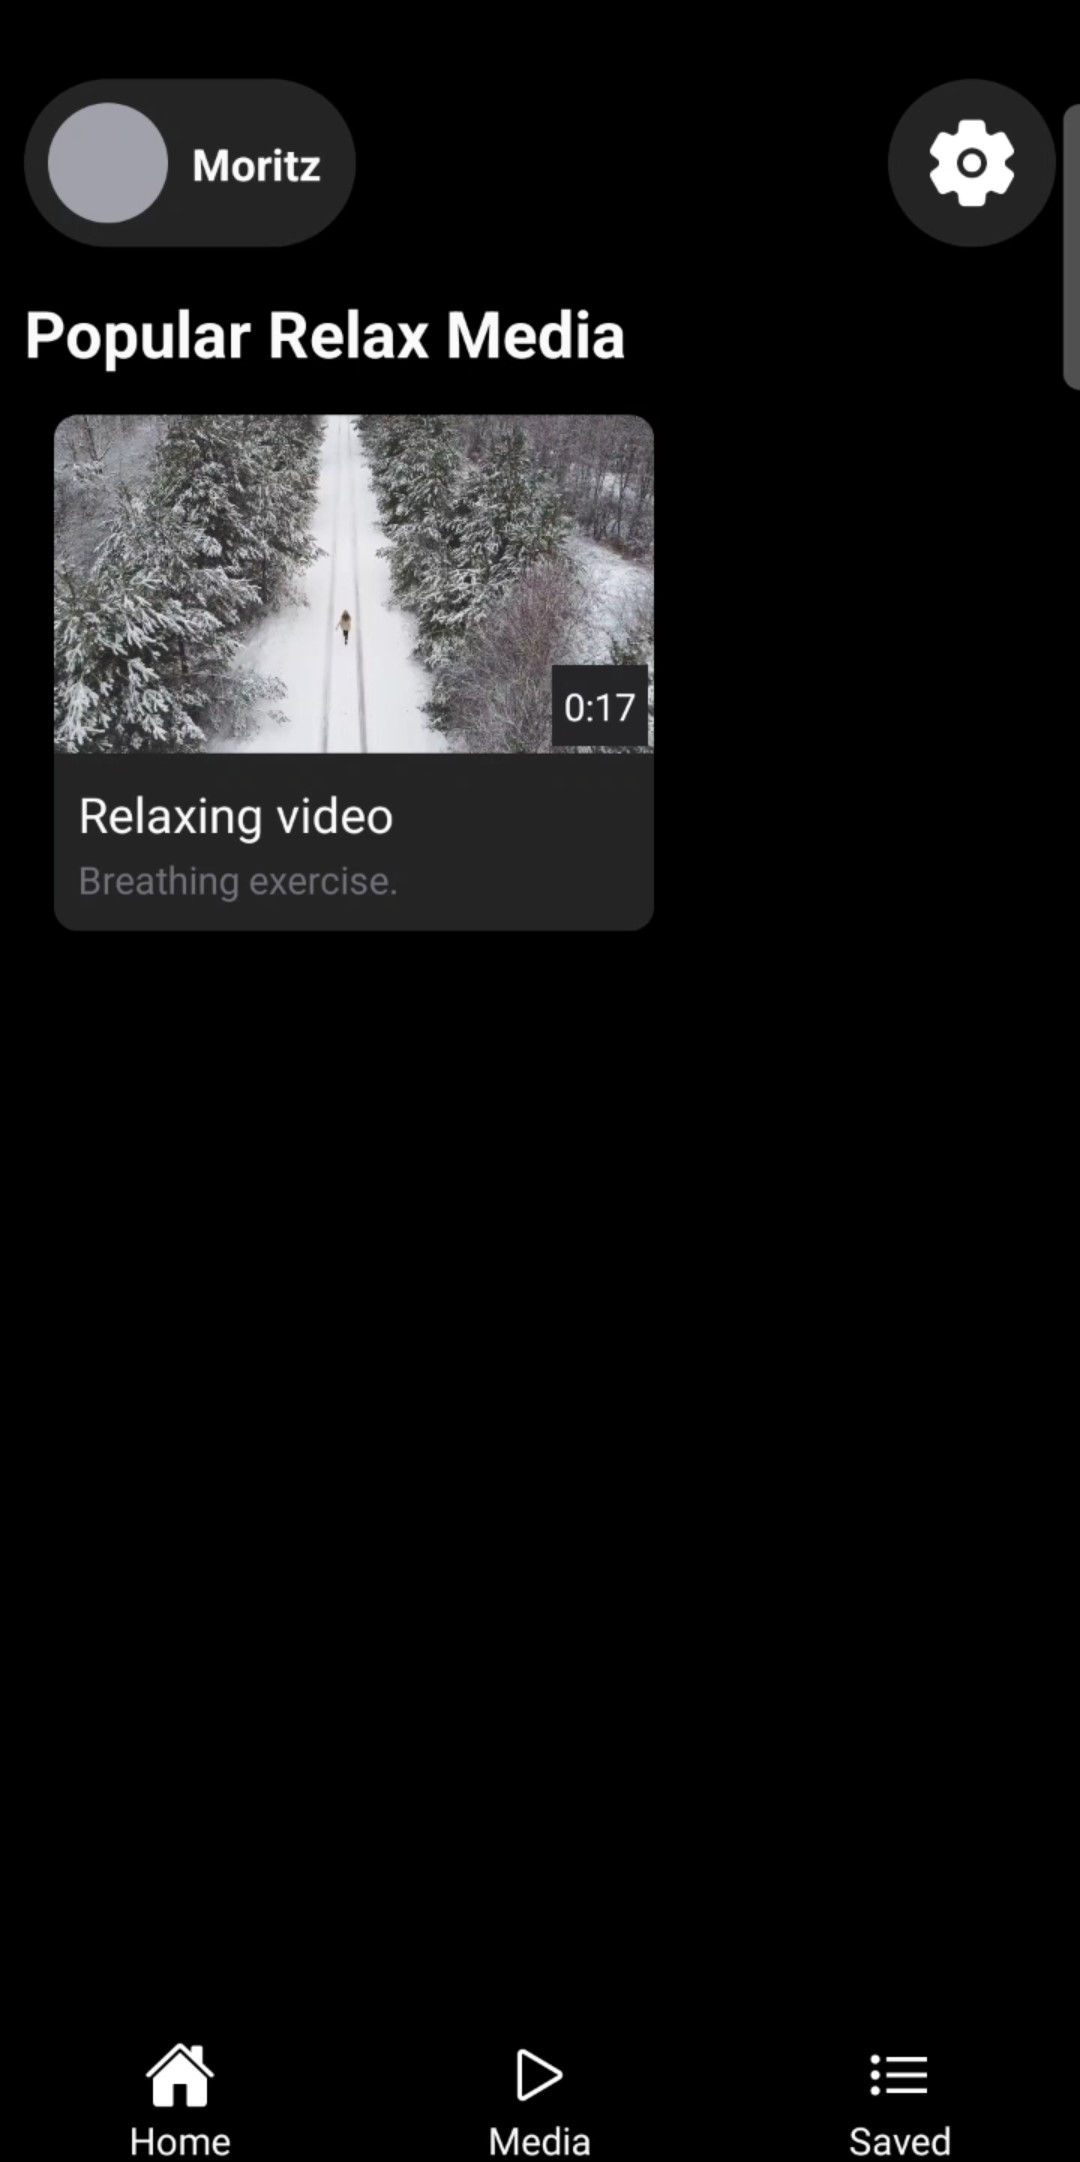
\includegraphics[height=2\textwidth]{./pics/dHome.jpg}
        \caption{Dark Home-Screen}
    \end{minipage}
    \begin{minipage}{0.5\textwidth}
        \centering
        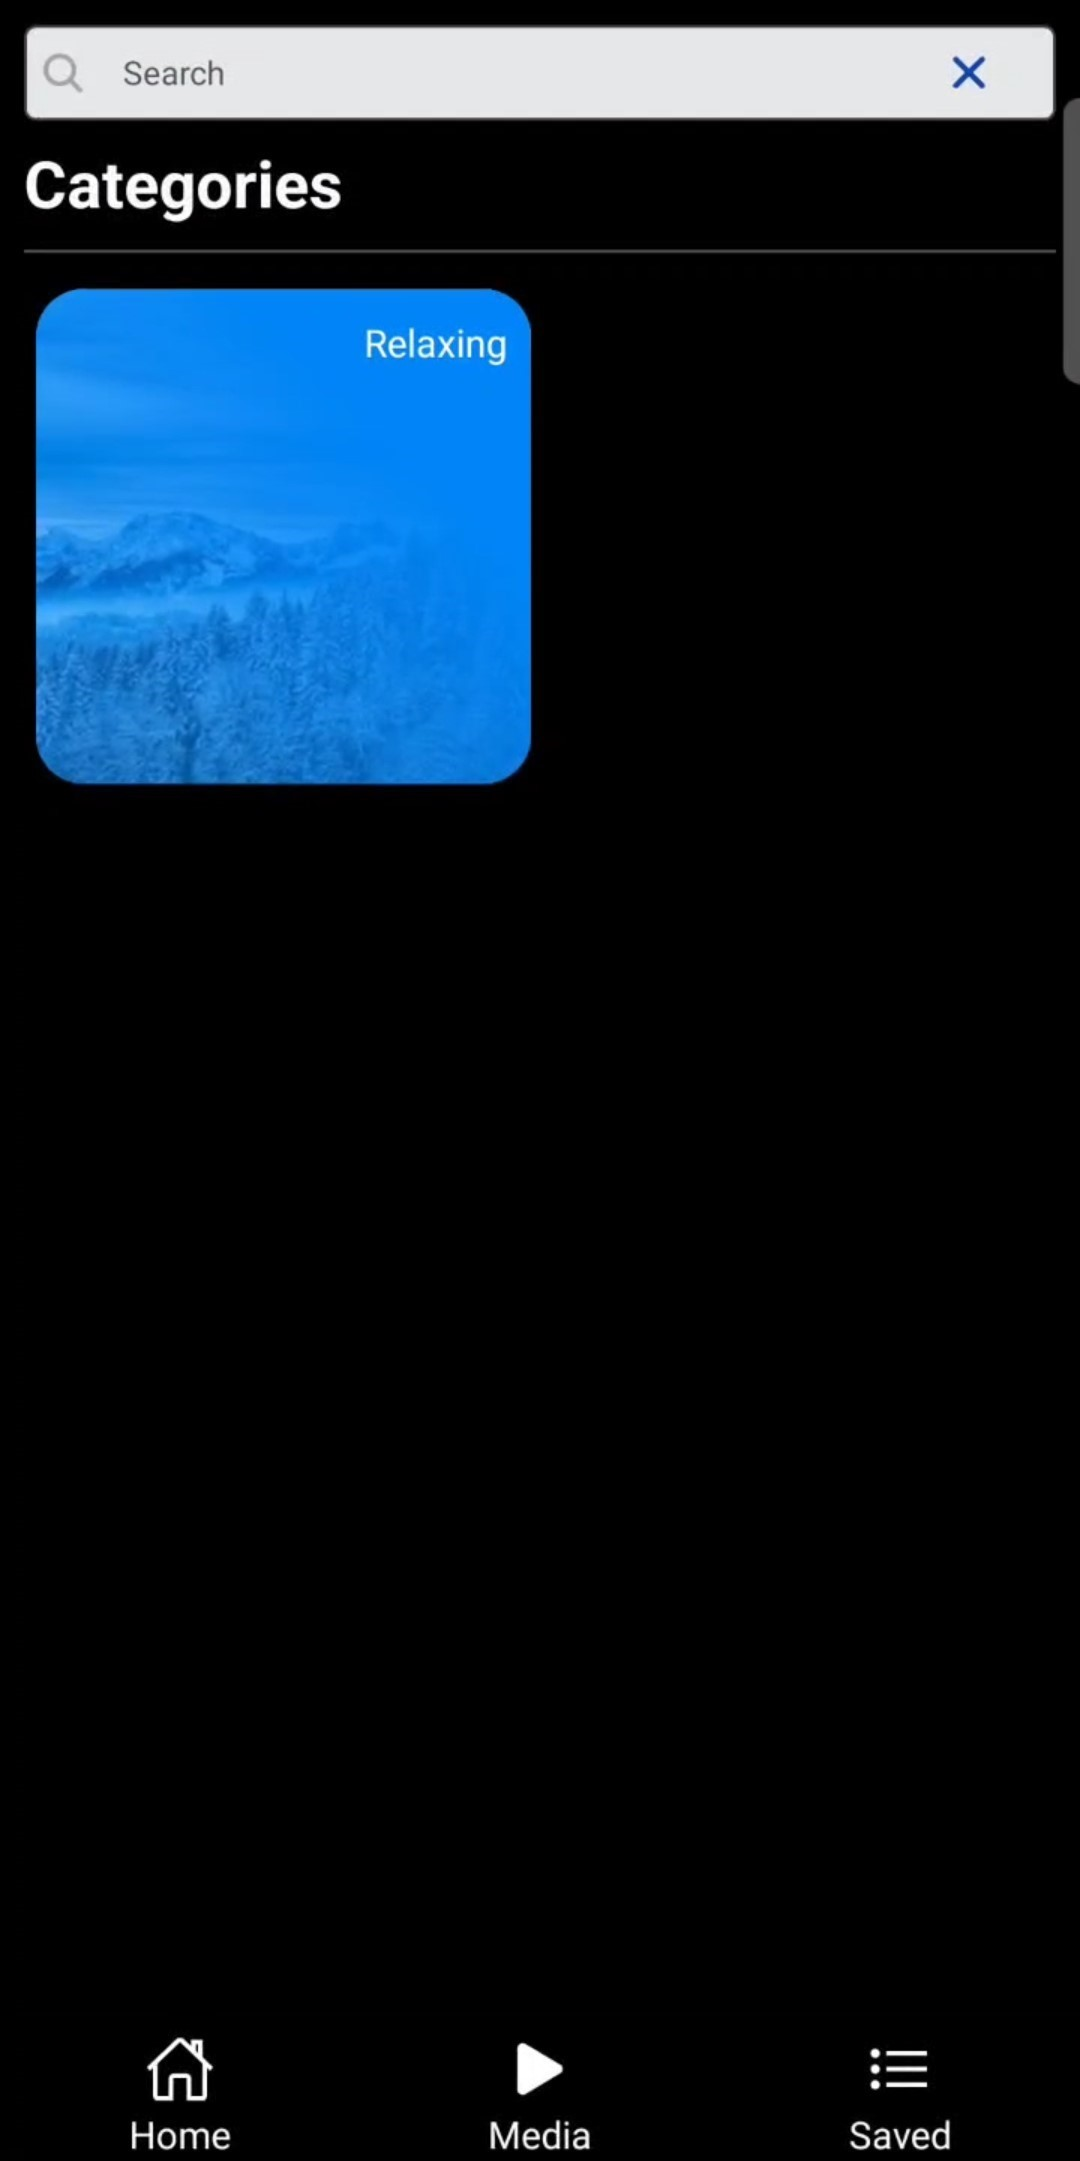
\includegraphics[height=2\textwidth]{./pics/dKategorie.jpg}
        \caption{Dark Kategorie-Screen}
    \end{minipage}
\end{figure}
\begin{figure}[H]
    \begin{minipage}{0.5\textwidth}
        \centering
        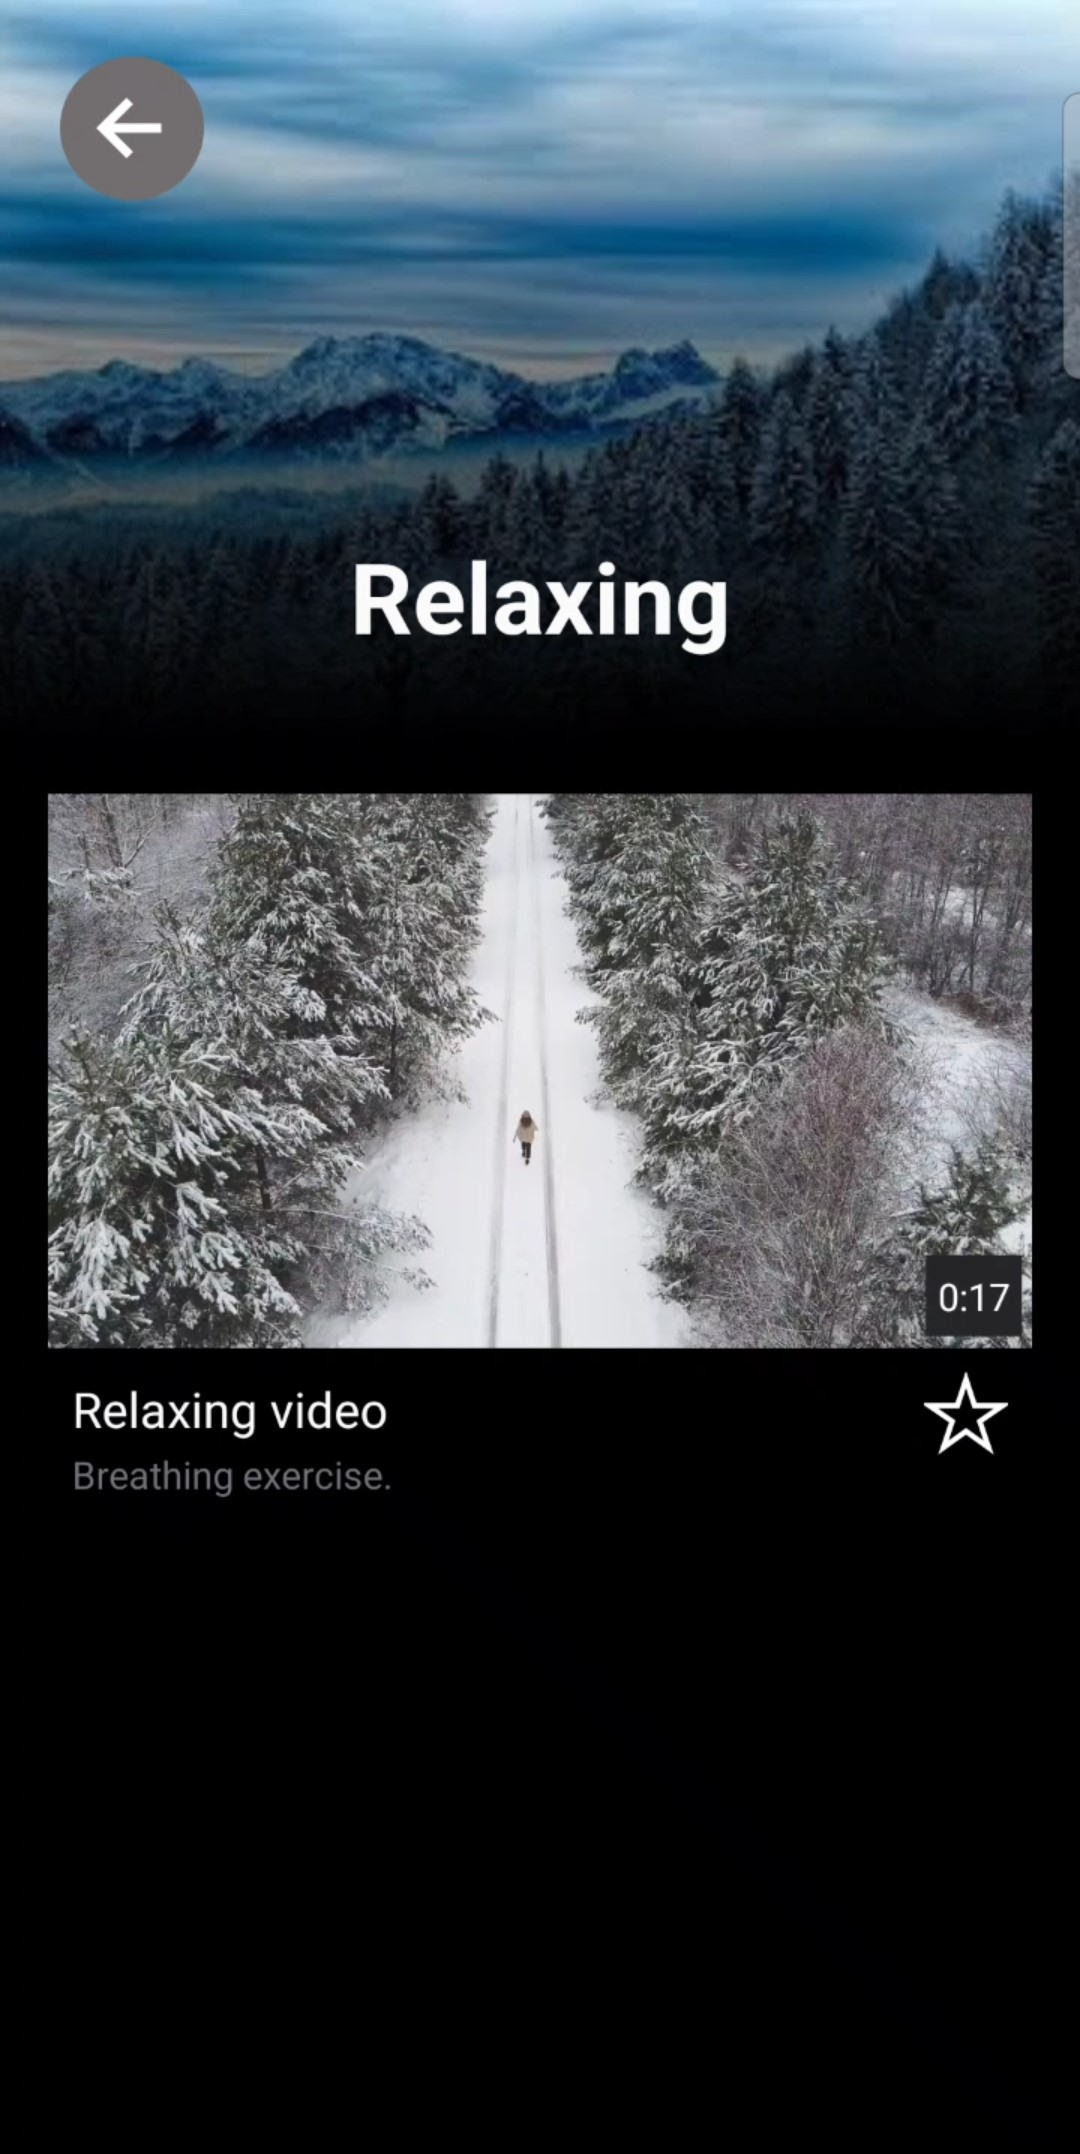
\includegraphics[height=1.9\textwidth]{./pics/dMedia.jpg}
        \caption{Dark Media-Screen}
    \end{minipage}
    \begin{minipage}{0.5\textwidth}
        \centering
        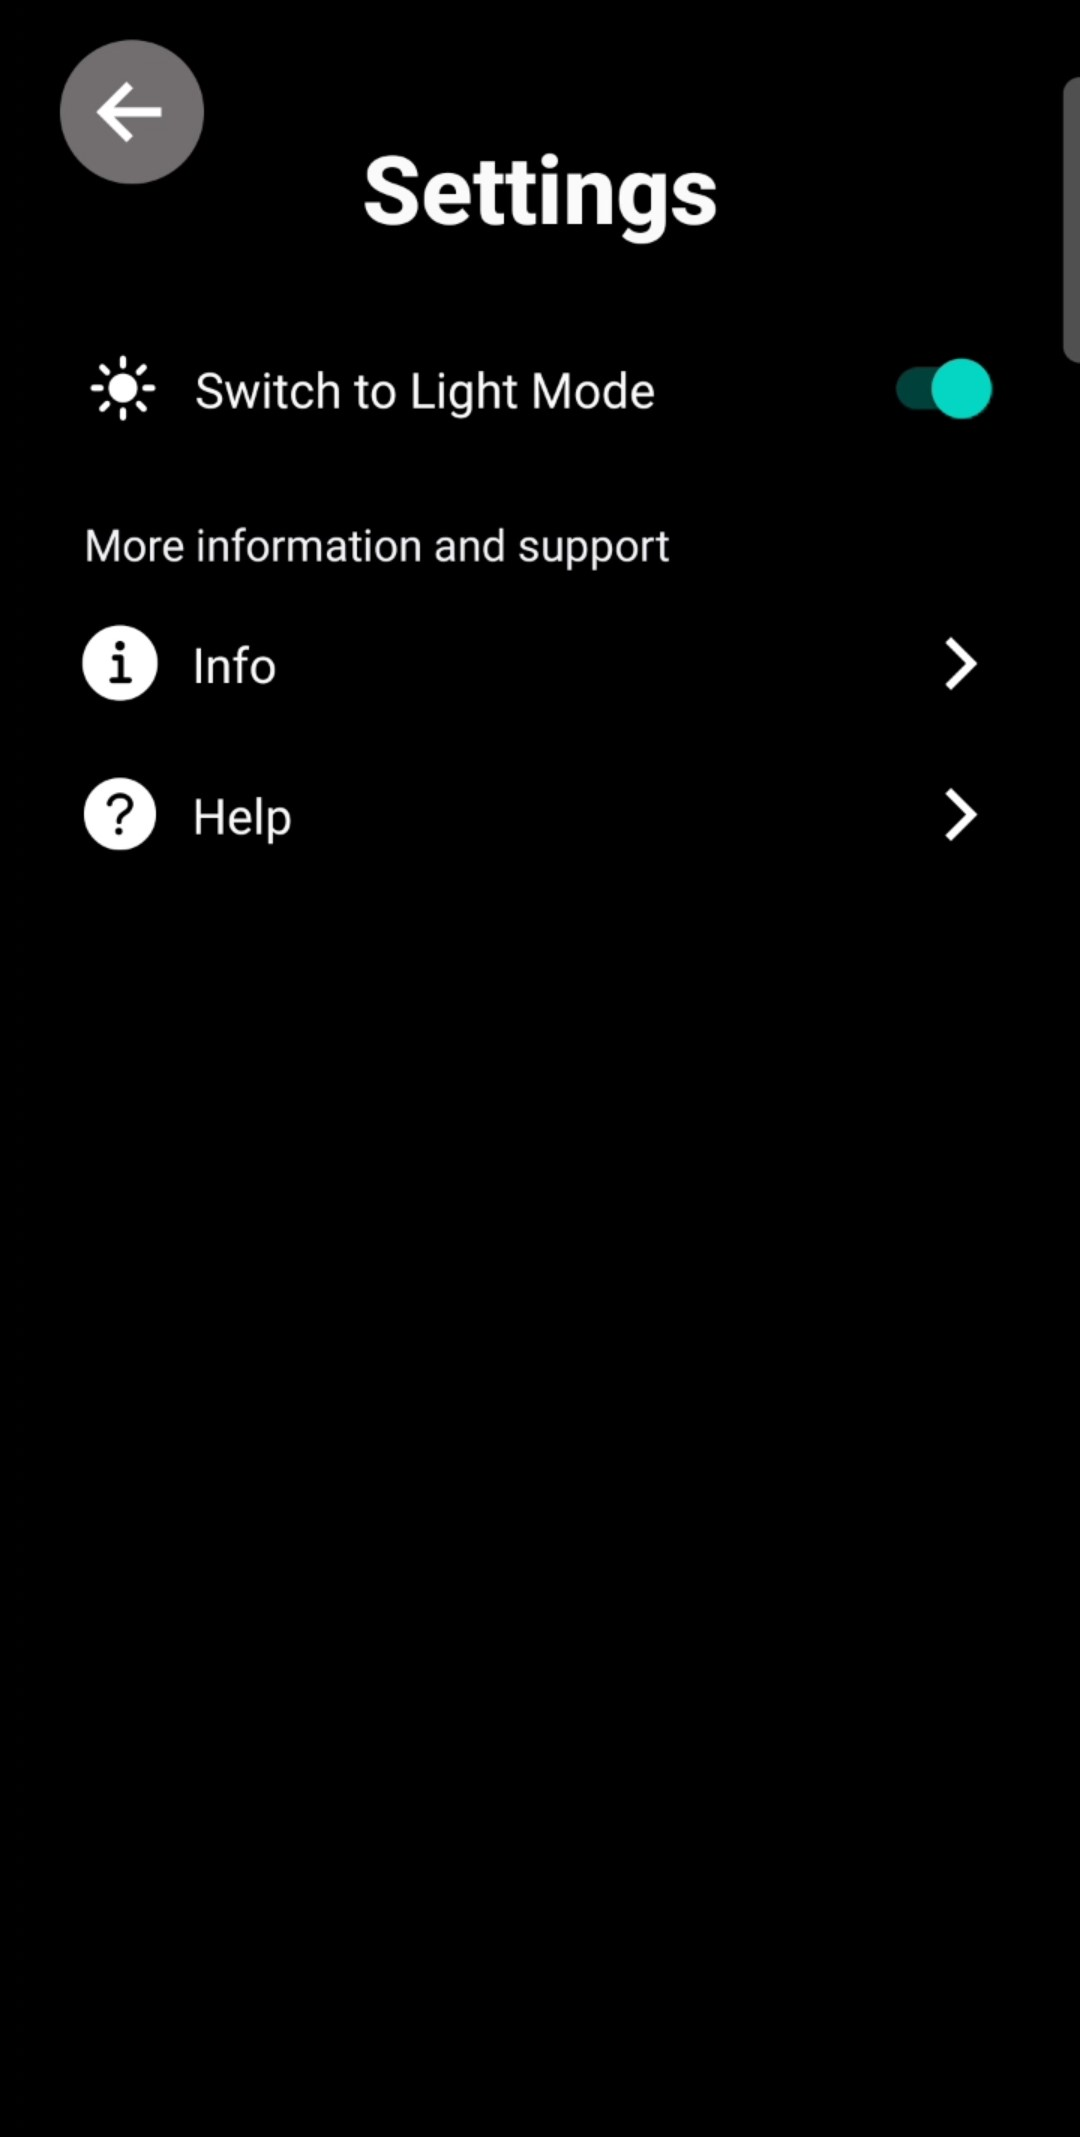
\includegraphics[height=1.9\textwidth]{./pics/dSettings.jpg}
        \caption{Dark Settings-Screen}
    \end{minipage}
\end{figure}

\newpage

\section{Logo}

Das Logo von Relaxoon besteht aus den beiden Buchstaben 'o', die stilisiert dargestellt sind. 
Es wird sowohl als App-Icon verwendet als auch im Google Play Store und im App Store angezeigt werden. Es gibt zwei 
Varianten des Logos: eine in Weiß und eine in Schwarz. Diese sind unten zu sehen.

\begin{figure}[H]
    \begin{minipage}{0.5\textwidth}
        \centering
        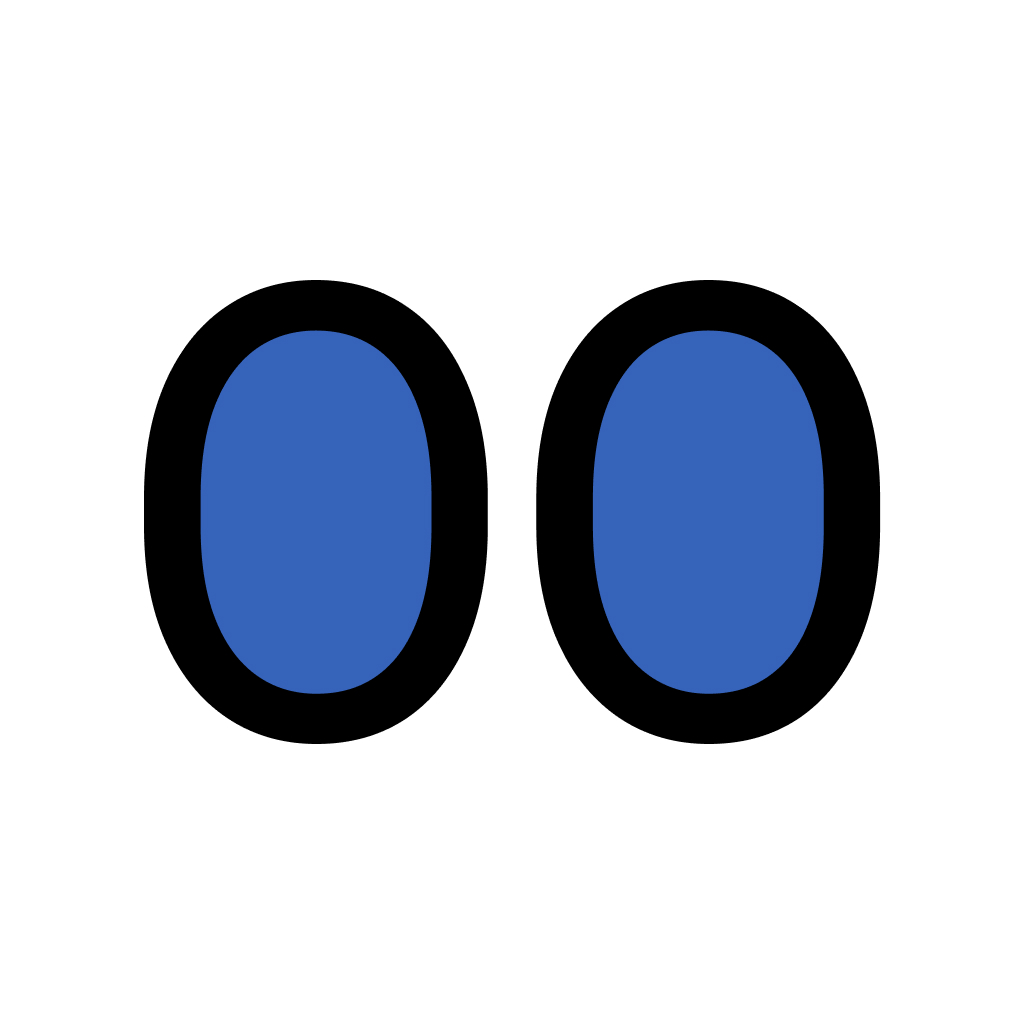
\includegraphics[height=0.8\textwidth]{./pics/Relaxoon Logo White.jpg}
        \caption{Logo in Weiß}
    \end{minipage}
    \begin{minipage}{0.5\textwidth}
        \centering
        
\includegraphics[height=0.8\textwidth]{./pics/Relaxoon Logo Black.jpg}
        \caption{Logo in Schwarz}
    \end{minipage}
\end{figure}